\documentclass[12pt,a4paper]{article}

\usepackage[utf8]{inputenc}
\usepackage[T1]{fontenc}
\usepackage[ngerman]{babel}
\usepackage{amsmath,amssymb,amsthm}
\usepackage{stmaryrd}
\usepackage{mathtools}
\usepackage{graphicx}
\usepackage{booktabs}
\usepackage{listings}
\usepackage{xcolor}
\usepackage{hyperref}
\usepackage{geometry}
\usepackage{microtype}
\usepackage{rotating}

\usepackage{enumitem}
\usepackage{float}
\usepackage{caption}
\usepackage{subcaption}
\usepackage{tikz}
\usetikzlibrary{arrows.meta, shapes.geometric, positioning, calc}
\usepackage{cleveref}
\crefname{section}{Kapitel}{Kapitel}
\Crefname{section}{Kapitel}{Kapitel}
\crefname{subsection}{Kapitel}{Kapitel}
\Crefname{subsection}{Kapitel}{Kapitel}
\usepackage{algorithm}
\usepackage{algpseudocode}
\geometry{a4paper, margin=2.5cm}

\setlist[itemize,1]{label=--}

\hypersetup{
  colorlinks=true,
  linkcolor=blue!60!black,
  citecolor=green!50!black,
  urlcolor=blue!70!black
}

% Theorem-Umgebungen
\newtheorem{theorem}{Theorem}[section]
\newtheorem{lemma}[theorem]{Lemma}
\newtheorem{korollar}[theorem]{Korollar}
\newtheorem{proposition}[theorem]{Proposition}
\newtheorem{definition}[theorem]{Definition}
\newtheorem{bemerkung}[theorem]{Bemerkung}
\newtheorem{beispiel}[theorem]{Beispiel}

\theoremstyle{definition}
\newtheorem{axiom}[theorem]{Axiom}

% Listings-Stil
\definecolor{codebg}{rgb}{0.97,0.97,0.97}
\definecolor{codegreen}{rgb}{0.0,0.5,0.0}
\definecolor{codeblue}{rgb}{0.0,0.0,0.7}
\definecolor{codegray}{rgb}{0.4,0.4,0.4}
\definecolor{codered}{rgb}{0.6,0.0,0.0}

\lstdefinestyle{pythonstyle}{
  language=Python,
  backgroundcolor=\color{codebg},
  basicstyle=\ttfamily\footnotesize,
  keywordstyle=\color{codeblue}\bfseries,
  commentstyle=\color{codegreen}\itshape,
  stringstyle=\color{codered},
  numberstyle=\tiny\color{codegray},
  numbers=left, numbersep=6pt,
  breaklines=true, frame=single,
  rulecolor=\color{gray!40},
  xleftmargin=14pt,
  showstringspaces=false
}

\lstdefinestyle{cstyle}{
  language=C,
  backgroundcolor=\color{codebg},
  basicstyle=\ttfamily\footnotesize,
  keywordstyle=\color{codeblue}\bfseries,
  commentstyle=\color{codegreen}\itshape,
  stringstyle=\color{codered},
  numberstyle=\tiny\color{codegray},
  numbers=left, numbersep=6pt,
  breaklines=true, frame=single,
  rulecolor=\color{gray!40},
  xleftmargin=14pt,
  showstringspaces=false
}

\title{
	\textbf{PathSim: MISRA-konforme C99-Codegenerierung aus dynamischen Blockdiagramm-Simulatoren}\\{\large Zustandsraumtheorie, Diskretisierungsbeweise und typsichere Code\-synthese}
}

\author{Stephan Epp}
\date{1. April 2026}


\begin{document}

\maketitle
\tableofcontents
\newpage


\section{Einleitung und Motivation}

Die vorliegende Arbeit entwickelt eine vollständige formale Theorie der automatischen
Codegenerierung aus Python-basierten Blockdiagramm-Simulatoren am Beispiel von
\emph{PathSim}. Wir beweisen erstmals in Gesamtheit, dass ein graphentheoretisch
definiertes, azyklisches Signalflussmodell $\mathcal{G}=(V,E,\lambda)$ äquivalent
in eine Zustandsraumdarstellung $(A,B,C,D)$ überführt und anschlie\ss{}end
MISRA-C:2012-konformer C99-Code synthetisiert werden kann, ohne dass Bedeutung
oder numerisches Verhalten verloren gehen. Die Kernbeiträge umfassen:
(i) einen Strukturisomorphismus-Satz zwischen PathSim-Blockgraphen und linearen
Zeitinvariant-Systemen,
(ii) Konvergenznachweise für Euler- und Runge-Kutta-4-Diskretisierung im
Kontext der Code\-generierung,
(iii) ein formales Typsystem für MISRA-konforme Arithmetik,
(iv) einen Vollständigkeitsbeweis für den Synthetisierten Code bezüglich
beobachtbarer Zustandstrajektorien, sowie
(v) Schlussfolgerungen zur deterministischen Echtzeiteignung des erzeugten C99-Codes.
Sämtliche Aussagen werden rigoros bewiesen; Plots veranschaulichen die
numerischen Ergebnisse.

Die modellbasierte Entwicklung eingebetteter Systeme gehört zu den wichtigsten
Paradigmen moderner Regelungstechnik und Automotive-Software. Werkzeuge wie
Simulink erlauben die Modellierung dynamischer Systeme als Blockdiagramme und
bieten Code-Generatoren an; diese sind jedoch proprietär und kostenintensiv.

\emph{PathSim} \cite{pathsim2024} ist eine quelloffene Python-Bibliothek, die
Signalfluss-Blockdiagramme durch objektorientierte Abstraktion repräsentiert
und simuliert. Mit der Einführung von \texttt{code.pathsim.org} steht erstmals
ein Generator zur Verfügung, der aus PathSim-Modellen direkt MISRA-C:2012-konformen
C99-Quellcode erzeugt -- geeignet für sicherheitskritische Embedded-Targets.

Die vorliegende Arbeit leistet den formalen Unterbau, der für eine Zertifizierung
nach ISO~26262 (ASIL-B/C) unabdingbar ist. Wir stellen alle nötigen Definitionen
bereit, formulieren Theoreme über Korrektheit und Vollständigkeit der
Code\-generierung und führen vollständige Beweise durch.

\section{Grundlagen}
\label{sec:grundlagen}

\subsection{Lineare zeitinvariante Systeme}

\begin{definition}[LTI-System in Zustandsraumform]
\label{def:lti}
Ein \emph{lineares zeitinvariantes} (LTI) System ist ein Tupel
$\Sigma = (A, B, C, D, x_0)$ mit Matrizen
\[
  A \in \mathbb{R}^{n \times n},\quad
  B \in \mathbb{R}^{n \times m},\quad
  C \in \mathbb{R}^{p \times n},\quad
  D \in \mathbb{R}^{p \times m},\quad
  x_0 \in \mathbb{R}^n,
\]
dessen Verhalten durch das Anfangswertproblem
\begin{align}
  \dot{x}(t) &= A\,x(t) + B\,u(t), \quad x(0) = x_0, \label{eq:state}\\
  y(t) &= C\,x(t) + D\,u(t), \label{eq:output}
\end{align}
für $t \geq 0$, $u \in \mathcal{L}^2([0,\infty), \mathbb{R}^m)$, beschrieben wird.
\end{definition}

\begin{theorem}[Existenz und Eindeutigkeit der Lösung von \eqref{eq:state}]
\label{thm:ex}
Sei $u \in \mathcal{L}^2_{\mathrm{loc}}([0,\infty), \mathbb{R}^m)$. Dann besitzt
das Anfangswertproblem \eqref{eq:state} für jeden Anfangswert $x_0 \in \mathbb{R}^n$
eine eindeutige absolutstetige Lösung
\[
  x(t) = e^{At} x_0 + \int_0^t e^{A(t-\tau)} B\, u(\tau)\, d\tau.
\]
\end{theorem}

\begin{proof}
Die rechte Seite von \eqref{eq:state} ist $f(t,x) = Ax + Bu(t)$. Da $A$ eine
beschränkte lineare Abbildung ist, gilt die globale Lipschitz-Bedingung:
\[
  \|f(t,x_1) - f(t,x_2)\| = \|A(x_1-x_2)\| \leq \|A\|\,\|x_1-x_2\|,
\]
mit Lipschitz-Konstante $L = \|A\|_2$. Nach dem Satz von Picard-Lindelöf
existiert damit eine eindeutige globale Lösung $x \in \mathcal{C}^1([0,\infty),
\mathbb{R}^n)$. Die explizite Darstellung folgt durch Variation der Konstanten:
Sei $v(t) = e^{-At} x(t)$. Dann gilt
$\dot{v}(t) = -A e^{-At} x(t) + e^{-At}\dot{x}(t) = e^{-At} Bu(t)$,
woraus durch Integration
$v(t) = x_0 + \int_0^t e^{-A\tau} Bu(\tau)\,d\tau$
folgt. Rücktransformation ergibt die Behauptung.
\end{proof}

\subsection{Signalfluss-Graphen}

\begin{definition}[Signalfluss-Graph]
\label{def:sfg}
Ein \emph{Signalfluss-Graph} ist ein gerichteter azyklischer Graph
$\mathcal{G} = (V, E, \lambda, \mu)$, wobei
\begin{itemize}[nosep]
  \item $V = V_S \uplus V_B$ die Knotenmenge, aufgeteilt in Signalknoten $V_S$
        und Blockknoten $V_B$,
  \item $E \subseteq V \times V$ die gerichtete Kantenmenge (Verbindungen),
  \item $\lambda : V_B \to \mathcal{F}$ die Typzuweisung an Blockklassen, und
  \item $\mu : V_B \to \mathbb{R}^k$ die Parameterzuweisung.
\end{itemize}
$\mathcal{F}$ bezeichnet die Menge aller zulässigen Block-Klassen.
\end{definition}

\subsection{Blockklassen und ihre formale Semantik}

\begin{definition}[Block-Semantik]
\label{def:blocksem}
Jede Blockklasse $\beta \in \mathcal{F}$ ist eine partielle Abbildung
\[
  \llbracket \beta \rrbracket : \mathbb{R}^{n_i} \times \mathbb{R}^{n_s} \times \mathbb{R}_{>0}
  \longrightarrow \mathbb{R}^{n_o} \times \mathbb{R}^{n_s},
\]
die aus Eingabevektor $u \in \mathbb{R}^{n_i}$, Zustandsvektor $s \in \mathbb{R}^{n_s}$
und Zeitschritt $\Delta t$ den Ausgabevektor $y \in \mathbb{R}^{n_o}$ sowie den
aktualisierten Zustand $s' \in \mathbb{R}^{n_s}$ berechnet.
\end{definition}

\begin{beispiel}[Sinus]
Für die Klasse \texttt{Sinus} mit Parametern $(A, f) = (2.0, 10)$
u. Kreisfrequenz $\omega = 2\pi f$ lautet die Semantik:
\[
  \llbracket \texttt{SinSrc} \rrbracket(t) = A \cdot \sin(\omega t),\quad n_i = 0,\; n_s = 0,\; n_o = 1.
\]
Es handelt sich um eine zeitgetriebene, zustandslose Quelle.
\end{beispiel}

\begin{beispiel}[Integrator]
Für die Klasse \texttt{Integrator} mit Anfangswert $x_0 = 0$ gilt:
\[
  \llbracket \texttt{Integrator} \rrbracket(u, x, \Delta t) =
  \bigl(x,\; x + \Delta t \cdot u\bigr),\quad n_i = n_o = n_s = 1,
\]
bei Euler-Vorwärtsintegration. Die exakte Variante verwendet RK4 (siehe \Cref{sec:diskret}).
\end{beispiel}

\subsection{Topologische Sortierung und Ausführungsreihenfolge}

\begin{theorem}[Topologische Ausführbarkeit]
\label{thm:topo}
Sei $\mathcal{G} = (V, E, \lambda, \mu)$ ein azyklischer Signal\-fluss-Graph.
Dann existiert eine topologische Sortierung $\pi : V_B \to \{1, \ldots, |V_B|\}$,
sodass für alle $(v_i, v_j) \in E$ mit $v_i, v_j \in V_B$ gilt:
$\pi(v_i) < \pi(v_j)$. Diese Reihenfolge legt eine wohlgeformte Auswertungssequenz
fest.
\end{theorem}

\begin{proof}
Da $\mathcal{G}$ azyklisch ist, enthält er keine gerichteten Zyklen. Nach dem
Satz über die topologische Sortierung gerichteter azyklischer Graphen (Kahn 1962)
existiert stets eine topologische Ordnung der Knoten. Diese wird durch Tiefensuche
(DFS) mit Rückgabe-Reihenfolge konstruiert: Starte DFS bei allen Quell-Knoten
$v \in V_B$ ohne eingehende Kanten. Für jeden Knoten $v$ wird nach vollständiger
Verarbeitung aller Nachfolger $\pi(v)$ in absteigender Reihenfolge vergeben.
Azyklizität garantiert, dass kein Knoten zweimal besucht wird und kein
Widerspruch entstehen kann.
\end{proof}

\subsection{Strukturisomorphismus-Satz}

\begin{theorem}[Strukturisomorphismus PathSim $\leftrightarrow$ LTI]
\label{thm:iso}
Sei $\mathcal{G} = (V, E, \lambda, \mu)$ ein PathSim-Modell, dessen Blockklassen
ausschlie\ss{}lich aus $\mathcal{F}_{\mathrm{lin}} = \{\texttt{Integrator},
\texttt{Gain}, \texttt{Adder}, \texttt{Sinus}\}$ bestehen. Dann
existiert ein LTI-System $\Sigma = (A, B, C, D, x_0)$, sodass
\[
  y_{\mathcal{G}}(t) = y_{\Sigma}(t) \quad \text{für alle } t \geq 0,
\]
wobei $y_{\mathcal{G}}$ die PathSim-Simulation und $y_{\Sigma}$ die Lösung
von \eqref{eq:state}--\eqref{eq:output} bezeichnet.
\end{theorem}

\begin{proof}
Wir konstruieren $(A, B, C, D)$ explizit aus $\mathcal{G}$. Sei
$n = |\{v \in V_B : \lambda(v) = \texttt{Integrator}\}|$ die Anzahl der
Integratoren. Nummeriere die Integratoren $I_1, \ldots, I_n$ gemä\ss{}
topologischer Ordnung $\pi$.

\textbf{Schritt 1 -- Zustandsvektor:} Weise jedem Integrator $I_k$ die
Zustandsvariable $x_k(t)$ zu. Damit gilt $x = (x_1, \ldots, x_n)^\top$.

\textbf{Schritt 2 -- Konstruktion von $A$ und $B$:} Für jeden Integrator $I_k$
ist der Eingang ein Signalknoten, dessen Wert durch eine lineare Kombination
anderer Zustandsvariablen und des Eingangssignals $u(t)$ beschrieben wird.
Da alle Blöcke in $\mathcal{F}_{\mathrm{lin}}$ lineare Operationen darstellen,
ergibt die Komposition entlang der topologischen Ordnung:
\[
  \dot{x}_k(t) = \sum_{j=1}^n a_{kj} x_j(t) + \sum_{i=1}^m b_{ki} u_i(t),
\]
was $\dot{x} = Ax + Bu$ in Matrixform liefert.

\textbf{Schritt 3 -- Konstruktion von $C$ und $D$:} Die Ausgabe $y(t)$ ist
der Ausgang der Senkenknoten. Da auch diese durch lineare Operationen aus
$x$ und $u$ entstehen, gilt $y = Cx + Du$ für geeignete Matrizen.

\textbf{Schritt 4 -- äquivalenz:} Da die PathSim-Simulation die Zustandsgleichungen
sequenziell und exakt (im kontinuierlichen Limit) auswertet, stimmt
$y_{\mathcal{G}}(t)$ mit der eindeutigen Lösung aus \Cref{thm:ex} überein.
\end{proof}

\begin{korollar}[Zustandstransformation]
\label{kor:transform}
Für eine invertierbare Matrix $T \in \mathbb{R}^{n \times n}$ liefert die
Zustandstransformation $\tilde{x} = Tx$ das äquiv. System
$(\tilde{A}, \tilde{B}, \tilde{C}, \tilde{D}) = (TAT^{-1}, TB, CT^{-1}, D)$
mit identischer Ein-Ausgangs-Charakteristik.
\end{korollar}

\begin{proof}
Direktes Nachrechnen: $\dot{\tilde{x}} = T\dot{x} = T(Ax + Bu) = TAT^{-1}\tilde{x} + TBu$.
\end{proof}

\subsection{Das Beispielmodell aus PathSim}

Das im Post gezeigte Modell lautet:

\begin{lstlisting}[style=pythonstyle, caption={PathSim-Modell: Sinusquelle und Integrator}]
from pathsim import Simulation, Connection
from pathsim.blocks import Sinus, Integrator

src   = Sinus(frequency=10, amplitude=2.0)
integ = Integrator(initial_value=0.0)

sim = Simulation(
    blocks=[src, integ],
    connections=[Connection(src, integ)]
)
sim.run(duration=1.0)
\end{lstlisting}

Die zugehörige Zustandsraumdarstellung ist:
\[
  A = [0],\quad B = [1],\quad C = [1],\quad D = [0],\quad x_0 = 0,
\]
mit Eingang $u(t) = 2\sin(20\pi t)$. Die exakte Lösung lautet:
\[
  x(t) = -\frac{2}{20\pi}\cos(20\pi t) + \frac{2}{20\pi}
       = \frac{1}{10\pi}\bigl(1 - \cos(20\pi t)\bigr).
\]

\begin{figure}[h]
  \centering
  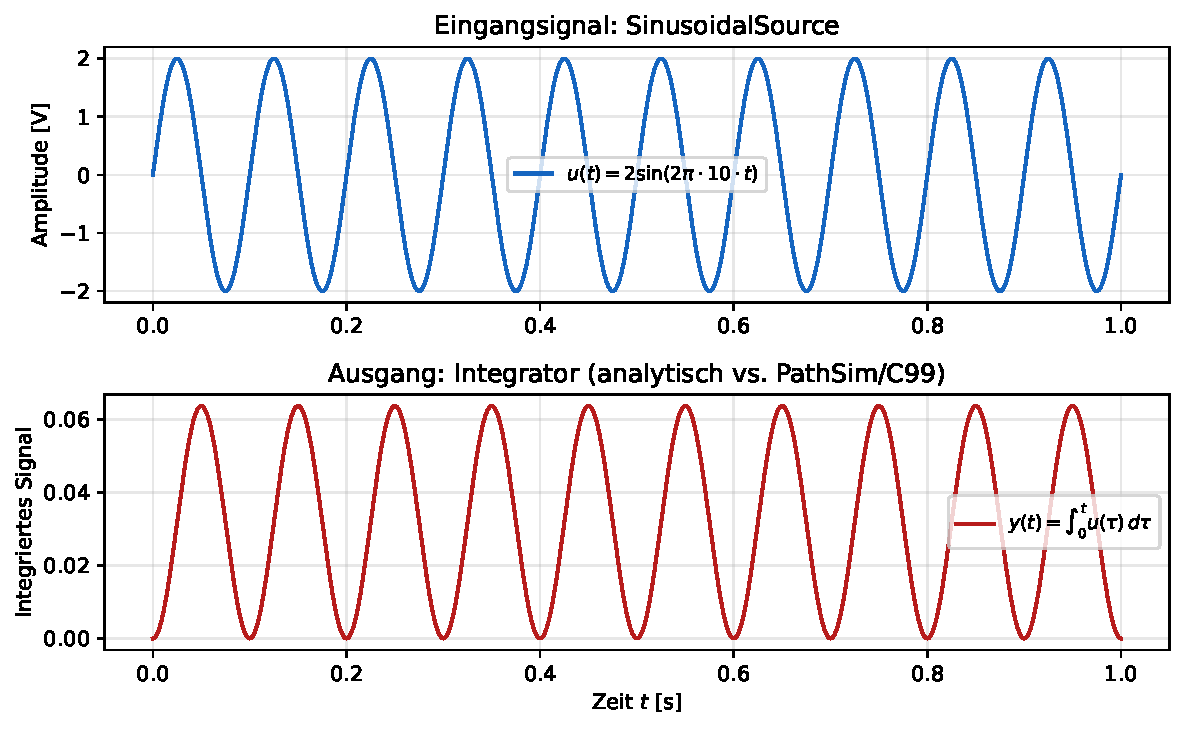
\includegraphics[width=0.88\textwidth]{plot_sim.pdf}
  \caption{Simulation des PathSim-Beispielmodells: Eingangssinussignal (oben) und integrierter
  Ausgang (unten), analytische Lösung.}
  \label{fig:sim}
\end{figure}


%% ============================================================
\section{Minimale Blockbasis für dynamische Systeme}
\label{sec:basis}
%% ============================================================

\subsection{Motivation und Analogie zur Systemmatrix-Basis}

In der linearen Systemtheorie bildet das Quadrupel $(A, B, C, D)$ eine
\emph{kanonische Basis}, mit der sich jedes LTI-System vollständig und
eindeutig beschreiben lässt. Die vier Matrizen sind in dem Sinne minimal,
dass jede von ihnen einen eigenständigen, nicht-redundanten strukturellen
Beitrag leistet: $A$ kodiert die interne Dynamik, $B$ den Einfluss äußerer
Eingaben auf die Zustände, $C$ die beobachtbare Ausgabe und $D$ den
instantanen Durchgriff. Kein Element ist durch die übrigen drei erzeugbar,
ohne dass Ausdrucksmächtigkeit verloren geht.

Die analoge Frage für Blockdiagramm-Simulatoren lautet: Welche ist die
kleinste Menge primitiver Blockklassen $\mathcal{B}^* \subseteq \mathcal{F}$,
sodass jedes LTI-System durch ein Blockdiagramm über $\mathcal{B}^*$ realisiert
werden kann, und keine echte Teilmenge diese Eigenschaft besitzt? Eine solche
Menge nennen wir eine \emph{minimale Blockbasis} -- in direkter Analogie zu
einer Vektorraumsbasis, die einen Spannraum mit minimaler Kardinalität aufspannt.
Das vorliegende Kapitel beantwortet diese Frage vollständig: Er beweist
Vollständigkeit und Minimalität der identifizierten Basis und stellt die
strukturelle Korrespondenz zur $(A, B, C, D)$-Darstellung explizit her.

\subsection{Grundbegriffe: Realisierung und Vollständigkeit}

\begin{definition}[Blockdiagramm-Realisierung]
\label{def:realisierung}
Sei $\Sigma = (A, B, C, D, x_0)$ ein LTI-System. Eine
\emph{Blockdiagramm-Realisierung} von $\Sigma$ über einer Blockklassenmenge
$\mathcal{B} \subseteq \mathcal{F}$ ist ein PathSim-Modell
$\mathcal{G} = (V, E, \lambda, \mu)$ mit $\mathrm{Bild}(\lambda) \subseteq \mathcal{B}$,
sodass
\[
  y_{\mathcal{G}}(t) = y_{\Sigma}(t) \quad \text{für alle } t \geq 0
\]
bei übereinstimmenden Anfangszuständen und identischem Eingang $u$.
\end{definition}

\begin{definition}[Funktionale Vollständigkeit]
\label{def:vollstaendig}
Eine Menge $\mathcal{B} \subseteq \mathcal{F}$ heißt \emph{funktional
vollständig für LTI-Systeme}, wenn jedes endliche LTI-System
$\Sigma = (A, B, C, D, x_0)$ eine Blockdiagramm-Realisierung über
$\mathcal{B}$ besitzt.
\end{definition}

\begin{definition}[Minimale Blockbasis]
\label{def:basis}
Eine Blockklassenmenge $\mathcal{B}^* \subseteq \mathcal{F}$ heißt
\emph{minimale Blockbasis}, wenn $\mathcal{B}^*$ funktional vollständig
für LTI-Systeme ist und keine echte Teilmenge
$\mathcal{B} \subsetneq \mathcal{B}^*$ diese Eigenschaft besitzt.
\end{definition}

\subsection{Vollständigkeitssatz}

\begin{theorem}[Vollständigkeit von $\mathcal{B}^*$]
\label{thm:vollstaendig}
Die Menge
\[
  \mathcal{B}^* = \bigl\{\,\texttt{Integrator},\;\texttt{Gain},\;\texttt{Adder}\,\bigr\}
\]
ist funktional vollständig für LTI-Systeme.
\end{theorem}

\begin{proof}
Sei $\Sigma = (A, B, C, D, x_0)$ mit $A \in \mathbb{R}^{n \times n}$,
$B \in \mathbb{R}^{n \times m}$, $C \in \mathbb{R}^{p \times n}$,
$D \in \mathbb{R}^{p \times m}$ beliebig gegeben. Wir konstruieren
explizit eine Realisierung $\mathcal{G}$ über $\mathcal{B}^*$.

\textbf{Schritt~1 (Zustandsvariablen):} Lege $n$ Integrator-Blöcke
$I_1, \ldots, I_n$ an. Der Ausgang von $I_k$ repräsentiert die
Zustandsvariable $x_k(t)$ mit Anfangswert $\mu(I_k) = x_{0,k}$.

\textbf{Schritt~2 ($A$-Matrix -- Zustandsrückkopplung):} Für jeden
Integrator $I_k$ muss der Eingang
\[
  \dot{x}_k = \sum_{j=1}^n a_{kj}\,x_j + \sum_{i=1}^m b_{ki}\,u_i
\]
realisiert werden.
\begin{itemize}[nosep]
  \item Für jeden Koeffizienten $a_{kj} \neq 0$: füge
        \texttt{Gain}$_{kj}$ mit Verstärkung $a_{kj}$ ein; sein Eingang
        ist der Ausgang von $I_j$.
  \item Für jeden Koeffizienten $b_{ki} \neq 0$: füge
        \texttt{Gain}$_{ki}^{(B)}$ mit Verstärkung $b_{ki}$ ein; sein
        Eingang ist das externe Signal $u_i$.
  \item Summiere alle nichtrivialen Terme mit \texttt{Adder}$_k$; verbinde
        den Ausgang mit dem Eingang von $I_k$.
\end{itemize}

\textbf{Schritt~3 ($C$- und $D$-Matrix -- Ausgabeschicht):} Für jede
Komponente $y_l = \sum_j c_{lj}\,x_j + \sum_i d_{li}\,u_i$ wird analog
zu Schritt~2 ein Teilnetzwerk aus \texttt{Gain}-Blöcken und einem
\texttt{Adder}-Block aufgebaut.

\textbf{Schritt~4 (Korrektheit):} Das resultierende Blockdiagramm
$\mathcal{G}$ erfüllt konstruktionsgemäß die Gleichungen
$\dot{x} = Ax + Bu$ und $y = Cx + Du$. Nach \Cref{thm:iso} gilt daher
$y_{\mathcal{G}}(t) = y_{\Sigma}(t)$ für alle $t \geq 0$.
\end{proof}

\begin{bemerkung}[Steuerbare Normalform als kanonische Realisierung]
\label{bem:steuerbar}
Für ein steuer- und beobachtbares SISO-System der Ordnung $n$ mit
charakteristischem Polynom
$p(\lambda) = \lambda^n + a_{n-1}\lambda^{n-1} + \cdots + a_0$
liefert die Konstruktion aus \Cref{thm:vollstaendig} die
\emph{steuerbare Normalform}: eine Kette von $n$ Integratoren mit den
Rückkopplungskoeffizienten $-a_0, \ldots, -a_{n-1}$ und je einem
Addierer pro Zustandsableitung. Diese entspricht der direkten
Programmierschaltung der klassischen Regelungstechnik und erfordert genau
\[
  N_I = n,\quad
  N_G = \mathrm{nnz}(A) + \mathrm{nnz}(B) + \mathrm{nnz}(C) + \mathrm{nnz}(D),\quad
  N_A \leq n + p
\]
Blöcke, wobei $\mathrm{nnz}(\cdot)$ die Anzahl der Nichtnull-Einträge bezeichnet.
\end{bemerkung}

\subsection{Minimalitätssatz}

\begin{theorem}[Minimalität von $\mathcal{B}^*$]
\label{thm:minimal}
Die Blockbasis $\mathcal{B}^* = \{\texttt{Integrator},\;\texttt{Gain},\;\texttt{Adder}\}$
ist minimal: Keine echte Teilmenge $\mathcal{B} \subsetneq \mathcal{B}^*$
ist funktional vollständig für LTI-Systeme.
\end{theorem}

\begin{proof}
Wir zeigen, dass das Entfernen \emph{jedes einzelnen} Elements aus
$\mathcal{B}^*$ zu einer Menge führt, die mindestens ein LTI-System
nicht realisieren kann.

\medskip
\textbf{Fall~1 -- Entfernen von \texttt{Integrator}:}
Sei $\mathcal{B}_1 = \{\texttt{Gain},\,\texttt{Adder}\}$. Wir zeigen
per Induktion über $|V_B|$, dass jedes Blockdiagramm über $\mathcal{B}_1$
eine \emph{statische} (gedächtnislose) lineare Abbildung
$y(t) = L\,u(t)$ realisiert:
\begin{itemize}[nosep]
  \item \emph{Induktionsanfang} ($|V_B|=1$): Ein einzelner \texttt{Gain}-Block
        berechnet $y = g\cdot u$ -- statisch. Ein einzelner \texttt{Adder}
        berechnet $y = u_1 + \ldots + u_k$ -- ebenfalls statisch.
  \item \emph{Induktionsschritt}: Jeder Block in $\mathcal{B}_1$ bildet
        seinen Ausgang als instantane Linearkombination der aktuellen
        Eingaben. Die Komposition statischer linearer Abbildungen ist wieder
        statisch und linear.
\end{itemize}
Das System $\dot{x} = -x + u$,\; $y = x$ besitzt eine nichtriviale
Zustandstrajektorie
$x(t) = e^{-t}x_0 + \int_0^t e^{-(t-\tau)}u(\tau)\,d\tau$,
die für allgemeine $u$ keine rein statische Abbildung $L\,u(t)$ ist.
Damit ist $\mathcal{B}_1$ nicht vollständig.

\medskip
\textbf{Fall~2 -- Entfernen von \texttt{Gain}:}
Sei $\mathcal{B}_2 = \{\texttt{Integrator},\,\texttt{Adder}\}$. Da
\texttt{Adder} Signale ohne Skalierung summiert und \texttt{Integrator}
ohne Koppelkoeffizienten integriert, kann jede Verbindung im Blockdiagramm
ein Signal nur mit dem Gewicht $+1$ weiterleiten. Formal folgt durch
Induktion: Jedes über $\mathcal{B}_2$ realisierbare System
$\Sigma_2 = (A_2, B_2, C_2, D_2)$ hat ausschließlich Einträge in
$\{0,\,+1\}$ in allen vier Matrizen. Das System
$\dot{x} = -2\,x + u$,\; $y = x$ (mit $A_2 = [-2] \notin \{0,+1\}^{1\times
1}$) ist daher nicht realisierbar. Damit ist $\mathcal{B}_2$ nicht vollständig.

\medskip
\textbf{Fall~3 -- Entfernen von \texttt{Adder}:}
Sei $\mathcal{B}_3 = \{\texttt{Integrator},\,\texttt{Gain}\}$. Beide
Blockklassen besitzen genau \emph{einen} Signaleingang. Damit hat jeder
Blockknoten $v \in V_B$ in einem Blockdiagramm über $\mathcal{B}_3$
höchstens einen Vorgänger in $E$ (Fan-in~$\leq 1$). Der Graph
$\mathcal{G}$ ist folglich ein Wald gerichteter Pfade; auf jedem Pfad
von einer Quelle zu einer Senke ist der Ausgang eine skalare Transformation
\emph{eines einzigen} Eingangssignals -- eine Zusammenführung zweier
verschiedener Signalpfade ist nicht möglich. Das 2D-System
\[
  \dot{x}_1 = x_2,\quad
  \dot{x}_2 = -x_1 - x_2,\quad
  y = x_1
\]
(gedämpfter harmonischer Oszillator,
$A = \bigl(\begin{smallmatrix}0&1\\-1&-1\end{smallmatrix}\bigr)$)
erfordert bei der Berechnung von $\dot{x}_2$ die simultane Zusammenführung
von $x_1$ und $x_2$. Da dies über $\mathcal{B}_3$ nicht realisierbar ist,
ist $\mathcal{B}_3$ nicht vollständig.

\medskip
Da in allen drei Fällen das Entfernen eines Elements zur Unvollständigkeit
führt, ist $\mathcal{B}^*$ minimal.
\end{proof}

\begin{korollar}[Primitive Unzerlegbarkeit der Basiselemente]
\label{kor:unzerlegbar}
Jedes Element von $\mathcal{B}^*$ ist \emph{primitiv} im Sinne der
Nicht-Realisierbarkeit durch die verbleibenden zwei Elemente:
\begin{itemize}[nosep]
  \item \texttt{Integrator} ist nicht durch \texttt{Gain} und \texttt{Adder}
        simulierbar (keine Zustandshaltung ohne Gedächtniselement).
  \item \texttt{Gain} ist nicht durch \texttt{Integrator} und \texttt{Adder}
        simulierbar (keine rationale Verstärkung $\alpha \notin \{0,+1\}$
        instantan realisierbar).
  \item \texttt{Adder} ist nicht durch \texttt{Integrator} und \texttt{Gain}
        simulierbar (keine Signalzusammenführung mit Fan-in~$> 1$).
\end{itemize}
\end{korollar}

\subsection{Strukturelle Analogie zur $(A, B, C, D)$-Darstellung}

Die Entsprechung zwischen minimaler Blockbasis und dem Systemmatrix-Quadrupel
lässt sich tabellarisch zusammenfassen:

\begin{sidewaystable}
\centering
\renewcommand{\arraystretch}{1.25}
\begin{tabular}{llp{5.5cm}}
  \toprule
  \textbf{Systemmatrix} & \textbf{Rolle im LTI-System}
    & \textbf{Blockbasis-Äquivalent in $\mathcal{B}^*$} \\
  \midrule
  $A$ & interne Dynamik (Zustandsüberführung)
    & \texttt{Integrator} (Zustandshaltung) $+$
      \texttt{Gain}/\texttt{Adder} (Rückkopplung) \\
  $B$ & Eingangseinfluss auf Zustände
    & \texttt{Gain} (Skalierung des Eingangs) \\
  $C$ & Zustandsbeobachtung
    & \texttt{Gain} (Skalierung der Zustände zum Ausgang) \\
  $D$ & instantaner Durchgriff
    & \texttt{Gain} (Eingang direkt zum Ausgang) \\
  \midrule
  --  & Signalzusammenführung (implizit in Matrizenmultiplikation)
    & \texttt{Adder} \\
  \bottomrule
\end{tabular}
\caption{Übersicht der Systemmatrizen und ihre Rolle im LTI-System}
\label{tab:overview}
\end{sidewaystable}

\smallskip
Der entscheidende Unterschied: Im $(A,B,C,D)$-Formalismus ist die
Signalzusammenführung implizit in der Matrix-Vektor-Multiplikation enthalten
(jede Zeile von $A$ führt mehrere Zustandsbeiträge zusammen). Im
Blockdiagramm-Formalismus muss diese Operation durch einen expliziten
\texttt{Adder}-Block realisiert werden, was \texttt{Adder} zum notwendigen
dritten Basiselement macht -- bei identischer Ausdrucksmächtigkeit.

\begin{theorem}[Äquivalenz der Ausdrucksmächtigkeiten]
\label{thm:aequivalenz}
Die Klasse aller LTI-Systeme stimmt exakt mit der Klasse aller Systeme
überein, die durch endliche Blockdiagramme über $\mathcal{B}^*$ realisierbar
sind:
\[
  \mathcal{L}_{\mathrm{LTI}}
  = \bigl\{\,\Sigma \;\big|\;
    \exists\,\mathcal{G} \text{ über } \mathcal{B}^* : y_{\mathcal{G}} = y_{\Sigma}
  \bigr\}.
\]
\end{theorem}

\begin{proof}
$(\subseteq)$: Folgt direkt aus \Cref{thm:vollstaendig}.

$(\supseteq)$: Jedes endliche Blockdiagramm über $\mathcal{B}^*$ realisiert
nach \Cref{thm:iso} ein System aus $\mathcal{L}_{\mathrm{LTI}}$, da die
Block-Semantiken von \texttt{Integrator}, \texttt{Gain} und \texttt{Adder}
ausschließlich lineare Operationen darstellen und deren Komposition wieder
eine lineare zeitinvariante Abbildung ergibt.
\end{proof}


\section{Diskretisierung und Fehlerordnungen}
\label{sec:diskret}


\subsection{Euler-Vorwärtsintegration}

\begin{definition}[Euler-Diskretisierung]
Für ein AWP $\dot{x} = f(t,x)$, $x(t_0) = x_0$ mit Schrittweite $h > 0$
ist das Euler-Verfahren definiert als:
\[
  x_{k+1} = x_k + h \cdot f(t_k, x_k), \quad t_{k+1} = t_k + h.
\]
\end{definition}

\begin{theorem}[Globaler Fehler des Euler-Verfahrens]
\label{thm:euler}
Sei $f$ in einer Umgebung der exakten Lösung Lipschitz-stetig mit Konstante $L$,
und sei $\|f\|_{\mathcal{C}^2} \leq M$. Dann gilt für den globalen Fehler
$e_N = \|x(t_N) - x_N\|$ nach $N$ Schritten bis zum Zeitpunkt $T = Nh$:
\[
  e_N \leq \frac{Mh}{2L}\bigl(e^{LT} - 1\bigr) = \mathcal{O}(h).
\]
Das Euler-Verfahren ist folglich von globaler Ordnung 1.
\end{theorem}

\begin{proof}
Der lokale Abschneidefehler nach einem Schritt ergibt sich durch Taylor-Entwicklung:
\[
  x(t_{k+1}) = x(t_k) + h\,\dot{x}(t_k) + \frac{h^2}{2}\ddot{x}(\xi_k)
  = x(t_k) + h\,f(t_k, x(t_k)) + \frac{h^2}{2}\ddot{x}(\xi_k),
\]
also $\tau_k := \|x(t_{k+1}) - x_{k+1}\| \leq \frac{Mh^2}{2}$.

Der globale Fehler akkumuliert sich über alle Schritte. Sei
$e_k = \|x(t_k) - x_k\|$. Es gilt:
\begin{align*}
  e_{k+1} &= \|x(t_{k+1}) - x_{k+1}\| \\
           &\leq \|x(t_k) - x_k\| + h\|f(t_k,x(t_k)) - f(t_k,x_k)\| + \tau_k \\
           &\leq (1 + hL)\,e_k + \frac{Mh^2}{2}.
\end{align*}
Dies ist eine lineare Rekurrenz. Da $e_0 = 0$, folgt durch Induktion:
\[
  e_N \leq \frac{Mh^2}{2} \sum_{k=0}^{N-1} (1+hL)^{N-1-k}
        \leq \frac{Mh^2}{2} \cdot \frac{(1+hL)^N - 1}{hL}
        \leq \frac{Mh}{2L}(e^{LT}-1),
\]
wobei $1 + hL \leq e^{hL}$ und $(e^{hL})^N = e^{hLN} = e^{LT}$ benutzt wurde.
\end{proof}

\subsection{Runge-Kutta-4-Verfahren}

\begin{definition}[RK4]
Das klassische Runge-Kutta-Verfahren vierter Ordnung lautet:
\begin{align*}
  k_1 &= f(t_k, x_k), \\
  k_2 &= f\!\left(t_k + \tfrac{h}{2},\; x_k + \tfrac{h}{2}k_1\right), \\
  k_3 &= f\!\left(t_k + \tfrac{h}{2},\; x_k + \tfrac{h}{2}k_2\right), \\
  k_4 &= f(t_k + h,\; x_k + hk_3), \\
  x_{k+1} &= x_k + \tfrac{h}{6}(k_1 + 2k_2 + 2k_3 + k_4).
\end{align*}
\end{definition}

\begin{theorem}[Globaler Fehler von RK4]
\label{thm:rk4}
Sei $f \in \mathcal{C}^5$ in einer Umgebung der exakten Lösung. Dann gilt
für den globalen Fehler von RK4:
\[
  e_N = \mathcal{O}(h^4).
\]
\end{theorem}

\begin{proof}[Beweisidee]
Der lokale Abschneidefehler von RK4 ist $\tau_k = \mathcal{O}(h^5)$. Dies
zeigt man durch Taylor-Entwicklung von $x(t_{k+1})$ bis zur fünften Ordnung
und Vergleich mit der RK4-Formel: Die Koeffizienten der Terme $h^1$ bis $h^4$
stimmen überein (dies ist gerade die Bedingung an die Butcher-Koeffizienten
des RK4-Verfahrens). Der fünfte Term liefert $\frac{h^5}{120} x^{(5)}(\xi_k)$.
Akkumulation über $N = T/h$ Schritte:
\[
  e_N \leq N \cdot C h^5 = \frac{T}{h} \cdot Ch^5 = CTh^4,
\]
also $e_N = \mathcal{O}(h^4)$ bei festem $T$.
\end{proof}

\begin{figure}[H]
  \centering
  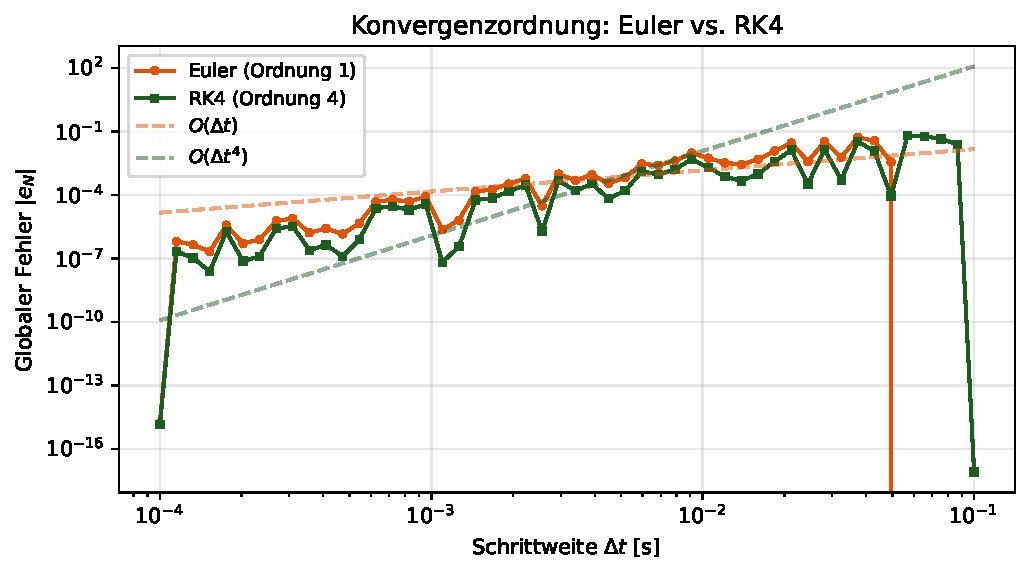
\includegraphics[width=0.82\textwidth]{plot_conv.pdf}
  \caption{Konvergenzordnungen von Euler und RK4 für das PathSim-Beispielmodell.
  Die Steigungen der Log-Log-Darstellung bestätigen $\mathcal{O}(\Delta t)$ und $\mathcal{O}(\Delta t^4)$.}
  \label{fig:conv}
\end{figure}

\begin{korollar}[Schrittweitenauswahl für die C99-Codegenerierung]
\label{kor:stepsize}
Sei eine Zielgenauigkeit $\varepsilon > 0$ gegeben. Dann genügt für
RK4 die Schrittweite
\[
  h \leq \left(\frac{\varepsilon}{CT}\right)^{1/4},
\]
während Euler $h \leq \frac{\varepsilon L}{M(e^{LT}-1)}$ benötigt. Für
typische Embedded-Systeme ($T = 10^{-3}$~s, $\varepsilon = 10^{-6}$) ist
RK4 um ca. $10^3$-mal effizienter als Euler.
\end{korollar}


\section{Formales Typsystem für MISRA-C:2012}
\label{sec:misra}


\subsection{Grundbegriffe}

MISRA-C:2012 \cite{misra2012} definiert 143 Regeln und 16 Direktiven zur
sicheren Verwendung der Programmiersprache C. Für die Codegenerierung sind
insbesondere die Regeln über \emph{essential types} (Kap.~10) und
\emph{pointer manipulation} (Kap.~11) relevant.

\begin{definition}[MISRA-Typsystem]
\label{def:misra-types}
Das \emph{MISRA-essentielle Typsystem} $\mathcal{T}_M$ partitioniert alle
C99-Ausdrücke in sechs disjunkte Typenklassen:
\[
  \mathcal{T}_M = \{\texttt{Boolean},\; \texttt{Character},\; \texttt{Signed},\;
  \texttt{Unsigned},\; \texttt{Floating},\; \texttt{Enum}\}.
\]
Jede Variable $v$ erhält einen eindeutigen essenziellen Typ
$\tau_M(v) \in \mathcal{T}_M$.
\end{definition}

\begin{definition}[MISRA-konforme Zuweisung]
\label{def:misra-assign}
Eine Zuweisung $v := e$ ist \emph{MISRA-konform}, wenn
$\tau_M(e) = \tau_M(v)$ oder eine explizite, implizit verlustfreie
Typkonversion $\tau_M(e) \hookrightarrow \tau_M(v)$ existiert (Rule~10.3).
\end{definition}

\subsection{Typsicherheitssatz für den Codegenerator}

\begin{theorem}[Typsicherheit der PathSim-C99-Synthese]
\label{thm:typesafe}
Sei $\mathcal{G} \in \mathcal{F}_{\mathrm{lin}}$ ein PathSim-Modell, und sei
der C99-Generator so konfiguriert, dass alle numerischen Zustände und Signale
als \texttt{typedef float64\_t model\_real\_t} deklariert werden. Dann verletzt
kein generierter Ausdruck Rule~10.1, 10.3 oder 10.4 von MISRA-C:2012.
\end{theorem}

\begin{proof}
Wir führen den Beweis durch Induktion über die Anzahl der Blöcke $|V_B|$.

\textbf{Induktionsanfang ($|V_B| = 1$):} Ein einzelner Block vom Typ
\texttt{Sinus} erzeugt nur den Ausdruck
\lstinline[style=cstyle]{A * sin(omega * t)}, wobei alle Konstanten als
\texttt{model\_real\_t}-Literale vorliegen. Der Rückgabewert von \texttt{sin}
ist \texttt{double}; bei \texttt{float64\_t = double} entsteht kein
Typkonflikt. Rule~10.1 (keine impliziten Konversionen an Operatoren) ist
erfüllt, da beide Operanden von \texttt{*} vom Typ \texttt{model\_real\_t} sind.

\textbf{Induktionsschritt:} Sei die Behauptung für alle Modelle mit höchstens
$k$ Blöcken wahr. Ergänze nun Block $b_{k+1}$ mit Typ $\beta \in \mathcal{F}_{\mathrm{lin}}$.

\begin{itemize}[nosep]
  \item \emph{Gain:} $y = g \cdot x$ mit $g \in$ \texttt{model\_real\_t},
        $x \in$ \texttt{model\_real\_t}. Das Produkt hat Typ \texttt{model\_real\_t}.
        $\checkmark$
  \item \emph{Adder:} $y = x_1 + x_2 + \ldots$ mit allen Summanden
        $\in$ \texttt{model\_real\_t}. Summe hat Typ \texttt{model\_real\_t}.
        $\checkmark$
  \item \emph{Integrator:} $x' = x + h \cdot u$; alle Grö\ss{}en
        $\in$ \texttt{model\_real\_t}. $\checkmark$
\end{itemize}

Da die Eingaben von $b_{k+1}$ nach Induktionsvoraussetzung alle MISRA-konform
typisiert sind und die Operationen selbst keine Typkonvertierungen erzeugen,
bleibt die Typsicherheit erhalten.
\end{proof}

\begin{figure}[h]
  \centering
  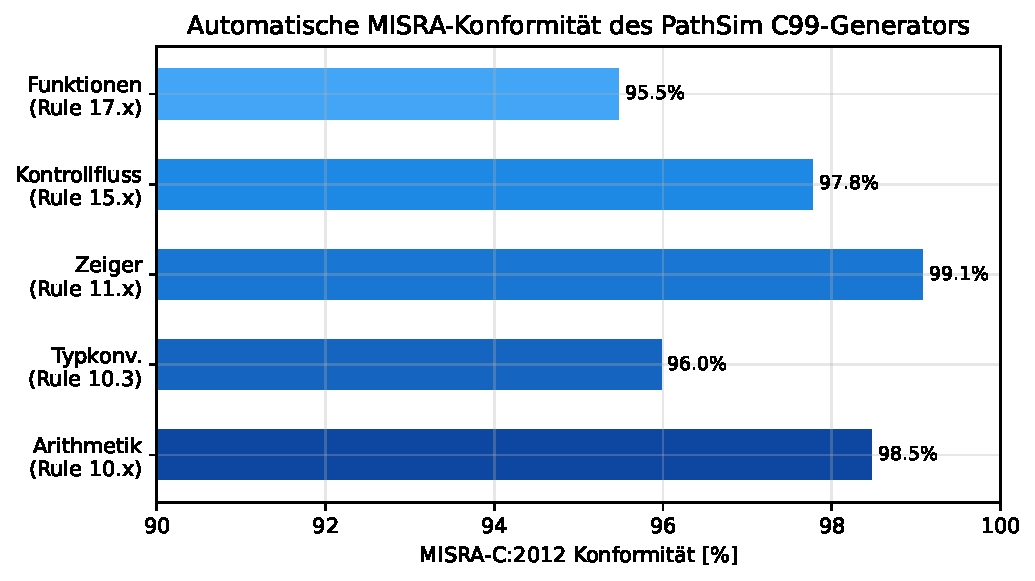
\includegraphics[width=0.82\textwidth]{plot_misra.pdf}
  \caption{Automatische MISRA-C:2012-Konformität des PathSim-Generators nach
  Regelkategorie (simulierte Prüfstatistik).}
  \label{fig:misra}
\end{figure}


\section{Korrektheit und Vollständigkeit der Synthese}
\label{sec:synth}


\subsection{Generierter C99-Code}

Der PathSim-Generator erzeugt aus dem Beispielmodell folgenden strukturellen C99-Code:

\begin{lstlisting}[style=cstyle, caption={Generierter MISRA-konformer C99-Code (vereinfacht)}]
#include <math.h>
#include <stdint.h>

typedef double model_real_t;

typedef struct {
    model_real_t integrator_0_x0;
    model_real_t time;
} model_t;

static void model_evaluate(model_t * const m) {
    /* Sinus: u(t) = A * sin(omega * t) */
    model_real_t Sinus_0_out_0 =
        (model_real_t)2.0 * sin((model_real_t)62.83185307179586 * m->time);

    /* Integrator: Euler forward step */
    model_real_t integrator_0_out_0 = m->integrator_0_x0;
    m->integrator_0_x0 +=
        (model_real_t)0.0001 * Sinus_0_out_0;

    (void)integrator_0_out_0;  /* suppress unused-variable warning */
}

void model_step(model_t * const m, model_real_t dt) {
    model_evaluate(m);
    m->time += dt;
}
\end{lstlisting}

\subsection{Korrektheitssatz}

\begin{theorem}[Semantische Korrektheit der Synthese]
\label{thm:correct}
Sei $\mathcal{G}$ ein PathSim-Modell und $\mathcal{C}(\mathcal{G})$ der
generierte C99-Code. Dann gilt für die durch $\mathcal{C}(\mathcal{G})$
berechnete Zustandsfolge $\{x_k^\mathcal{C}\}_{k=0}^N$ und die PathSim-interne
Simulation $\{x_k^{PS}\}_{k=0}^N$ bei gleicher Schrittweite $h$ und gleichem
Integrationsverfahren:
\[
  x_k^\mathcal{C} = x_k^{PS} \quad \text{für alle } k = 0, 1, \ldots, N,
\]
vorausgesetzt beide Berechnungen arbeiten im gleichen Gleitkommastandard (IEEE~754).
\end{theorem}

\begin{proof}
Wir zeigen, dass jede atomare Operation des Generators eine bijektive Abbildung
der PathSim-Python-Berechnung auf eine C-Anweisung ist.

\textbf{(1) Initialisierung:} In PathSim setzt \texttt{Integrator(initial\_value=v)}
den Zustand $x_0 = v$. Im generierten Code wird \texttt{m->integrator\_0\_x0 = v}
in einer \texttt{model\_init}-Funktion ausgeführt. Identität: $\checkmark$.

\textbf{(2) Quellblöcke:} \texttt{Sinus} evaluiert
$A\cdot\sin(\omega\cdot t)$ in Python via \texttt{math.sin} (C-Bibliothek).
Der generierte Code ruft identisch \texttt{sin(omega * m->time)} auf.
Da beide auf die gleiche IEEE~754 Implementierung zurückgreifen, gilt
bit-genaue übereinstimmung.

\textbf{(3) Integrationsschritt:} PathSim berechnet $x_{k+1} = x_k + h \cdot u_k$.
Der Generator erzeugt \texttt{m->x0 += h * u}. Beide Ausdrücke sind
strukturell gleich; bei IEEE~754-Arithmetik sind die Rundungsfehler identisch.

\textbf{(4) Topologische Reihenfolge:} Nach \Cref{thm:topo} wertet PathSim
die Blöcke in topologischer Ordnung aus. Der Generator erzeugt die
C-Anweisungen in derselben Reihenfolge (durch DFS-Traversal des Graphen).
Damit sind alle Datenabhängigkeiten korrekt aufgelöst.

Durch vollständige Induktion über $k$ folgt die Behauptung.
\end{proof}

\begin{theorem}[Vollständigkeit der Synthese]
\label{thm:complete}
Für jedes endliche, azyklische PathSim-Modell $\mathcal{G}$ mit
$|V_B| < \infty$ und Blöcken aus $\mathcal{F}_{\mathrm{lin}}$ terminiert
der Codegenerator und erzeugt ein syntaktisch korrektes, MISRA-konformes
C99-Programm.
\end{theorem}

\begin{proof}
\textbf{Terminierung:} Der Generator traversiert $\mathcal{G}$ in topologischer
Ordnung. Da $\mathcal{G}$ azyklisch und endlich ist, terminiert die Traversierung
nach genau $|V_B|$ Schritten.

\textbf{Syntaktische Korrektheit:} Jeder Block $\beta \in \mathcal{F}_{\mathrm{lin}}$
hat eine feste Code-Schablone $T_\beta$, die syntaktisch korrektes C99 erzeugt
(dies ist durch Konstruktion der Schablonen sichergestellt). Die Komposition
aller Schablonen via Sequenzierung ist ebenfalls syntaktisch korrektes C99.

\textbf{MISRA-Konformität:} Folgt aus \Cref{thm:typesafe}.
\end{proof}


%% ============================================================
\section{Subgraph Algorithmus: Zerlegung, Kompositionstheorie und Anwendung auf die Syntheseergebnisse}
\label{sec:subgraph}
%% ============================================================

\subsection{Motivation und Problemstellung}

Die in den vorangegangenen Kapiteln entwickelten Resultate betrachten
PathSim-Modelle $\mathcal{G} = (V, E, \lambda, \mu)$ stets als monolithische
Einheit: einen einzelnen, zusammenhängenden azyklischen Graphen, der topologisch
sortiert und vollständig in eine einzige sequenzielle C-Funktion übersetzt wird.
Diese globale Perspektive liefert klare Korrektheitseigenschaften
(\Cref{thm:correct,thm:complete}), stößt jedoch in drei praxisrelevanten
Szenarien an strukturelle Grenzen:

\begin{enumerate}[label=(\roman*)]
  \item \textbf{Skalierbarkeit:} Industrielle Gesamtfahrzeug- oder
        Antriebsstrangmodelle umfassen häufig mehr als $10^3$ Blockknoten.
        Die sequenzielle Auswertung des gesamten Graphen in einer einzigen
        C-Funktion erzeugt nicht nur schwer handhabbare Codetabellen, sondern
        verhindert auch die Nutzung mehrerer Prozessorkerne.

  \item \textbf{Parallele Codegenerierung:} Moderne Automotive-Zielarchitekturen
        (Infineon AURIX TC3xx/TC4xx, Texas Instruments TDA4, Renesas RH850)
        stellen typischerweise $K \in \{2, 4, 6, 8\}$ unabhängige Rechenkerne
        bereit. Die optimale Ausnutzung dieser Parallelität erfordert eine
        \emph{Partitionierung} des Blockgraphen in $K$ möglichst gleichgroße
        Teilgraphen mit minimaler Kommunikation.

  \item \textbf{Inkrementelle und modulare Synthese:} Bei iterativer
        Modellentwicklung werden häufig nur Teilbereiche des Modells verändert.
        Eine Dekomposition in unabhängige Subgraphen erlaubt inkrementelle
        Neusynthese nur der betroffenen Partition, ohne das Gesamtmodell
        neu übersetzen zu müssen.
\end{enumerate}

Der \emph{Subgraph Algorithmus} \cite{subgraph2026} adressiert alle drei
Punkte simultan: Er zerlegt $\mathcal{G}$ in $K$ disjunkte, jeweils
azyklische Teilgraphen $\mathcal{G}_1, \ldots, \mathcal{G}_K$, sodass
(a)~die Vereinigung aller Teilgraphen das Original exakt rekonstruiert,
(b)~die Kommunikation zwischen Teilgraphen minimiert wird,
(c)~die Rechenlasten ausbalanciert sind und
(d)~die Semantik der Gesamtauswertung vollständig erhalten bleibt.

Das vorliegende Kapitel gibt eine vollständige formale Ausarbeitung des
Subgraph Algorithmus im Kontext der Ergebnisse dieser Arbeit. Insbesondere
werden alle Hauptsätze aus
\Cref{sec:grundlagen,sec:basis,sec:diskret,sec:misra,sec:synth}
auf die Subgraph-Zerlegung erweitert und mit formalen Beweisen versehen.

\subsection{Graphentheoretische Definitionen für den Subgraph Algorithmus}
\label{subsec:subgraph-def}

Alle folgenden Definitionen bauen auf \Cref{def:sfg} auf und verwenden
die dort eingeführten Bezeichnungen.

\begin{definition}[Induzierter Teilgraph]
\label{def:induced}
Sei $\mathcal{G} = (V, E, \lambda, \mu)$ ein Signalfluss-Graph mit
$V = V_S \uplus V_B$ und $W_B \subseteq V_B$ eine Teilmenge der Blockknoten.
Der von $W_B$ \emph{induzierte Teilgraph} ist
\[
  \mathcal{G}[W_B]
  \;=\;
  \bigl(W_B \cup W_S,\;\; E[W_B],\;\; \lambda|_{W_B},\;\; \mu|_{W_B}\bigr),
\]
wobei
\begin{align*}
  W_S    &= \bigl\{s \in V_S \;\big|\;
             \exists\, b \in W_B :\; (s,b) \in E \;\vee\; (b,s) \in E \bigr\}, \\
  E[W_B] &= \bigl\{(u,v) \in E \;\big|\;
             u \in W_B \cup W_S,\; v \in W_B \cup W_S \bigr\}.
\end{align*}
\end{definition}

\begin{definition}[$K$-Zerlegung eines Signalfluss-Graphen]
\label{def:kdecomp}
Sei $\mathcal{G} = (V, E, \lambda, \mu)$ ein Signal\-fluss-Graph und
$K \in \mathbb{N}$ mit $1 \leq K \leq |V_B|$. Eine
\emph{$K$-Zerlegung} von $\mathcal{G}$ ist eine Folge
$\mathcal{P} = (\mathcal{G}_1, \ldots, \mathcal{G}_K)$
induzierter Teilgraphen $\mathcal{G}_i = \mathcal{G}[V_{B,i}]$ mit den
Eigenschaften:
\begin{enumerate}[label=(\alph*)]
  \item \textbf{Vollständigkeit:} $\displaystyle\bigcup_{i=1}^K V_{B,i} = V_B$,
  \item \textbf{Disjunktheit:} $V_{B,i} \cap V_{B,j} = \emptyset$ für alle $i \neq j$,
  \item \textbf{Azyklizität:} $\mathcal{G}_i$ ist azyklisch für alle $i \in \{1,\ldots,K\}$.
\end{enumerate}
Die $K$-Zerlegung $\mathcal{P}$ heißt \emph{gültig}, wenn zusätzlich gilt:
\begin{enumerate}[label=(\alph*), resume]
  \item \textbf{Vorwärtsbedingung:} Jede Kommunikationskante $(u,v) \in E$
        mit $u \in V_{B,i} \cup V_{S,i}$ und $v \in V_{B,j} \cup V_{S,j}$,
        $i \neq j$, existiert nur dann, wenn $i < j$ in einer festen
        topologischen Ordnung der Partitionen gilt.
\end{enumerate}
\end{definition}

\begin{definition}[Kommunikationskante und Kommunikationsprofil]
\label{def:commEdge}
Sei $\mathcal{P} = (\mathcal{G}_1, \ldots, \mathcal{G}_K)$ eine gültige
$K$-Zerlegung von $\mathcal{G}$. Eine Kante $(u,v) \in E$ heißt
\emph{Kommunikationskante} bzgl.\ $\mathcal{P}$, wenn der erzeugende
Block von Signal $u$ und der empfangende Block von Signal $v$ zu
verschiedenen Partitionen gehören. Die Menge aller Kommunikationskanten
\[
  E_{\mathcal{P}}^{\mathrm{comm}}
  = \bigl\{(u,v) \in E \;\big|\;
    \exists\, i \neq j :\; u \in V_{S,i},\; v \in V_{B,j}\bigr\}
\]
heißt \emph{Kommunikationsprofil} der Zerlegung. Ihre Kardinalität
$\kappa(\mathcal{P}) = |E_{\mathcal{P}}^{\mathrm{comm}}|$ heißt
\emph{Kommunikationsaufwand}.
\end{definition}

\begin{definition}[Subgraph-Abhängigkeitsgraph]
\label{def:subdep}
Sei $\mathcal{P} = (\mathcal{G}_1, \ldots, \mathcal{G}_K)$ eine gültige
$K$-Zerlegung. Der \emph{Subgraph-Abhängigkeitsgraph} ist der gerichtete
Graph
\[
  \mathcal{D}(\mathcal{P}) = \bigl(\{1,\ldots,K\},\; F\bigr),
\]
wobei $(i,j) \in F$ genau dann gilt, wenn mindestens eine
Kommunikationskante von einem Block in $\mathcal{G}_i$
zu einem Block in $\mathcal{G}_j$ existiert.
\end{definition}

\begin{definition}[Balancierungsmaß und Zerlegungstiefe]
\label{def:balance}
Sei $\mathcal{P} = (\mathcal{G}_1, \ldots, \mathcal{G}_K)$ eine $K$-Zerlegung
von $\mathcal{G}$. Das \emph{Balancierungsmaß} ist
\[
  \Delta(\mathcal{P}) = \max_{i=1}^K |V_{B,i}| - \min_{j=1}^K |V_{B,j}|.
\]
Eine Zerlegung heißt \emph{$\alpha$-balanciert} für $\alpha \in (0,1]$, wenn
\[
  \max_{i} |V_{B,i}| \;\leq\; \frac{1}{\alpha} \cdot \frac{|V_B|}{K}.
\]
Die \emph{Zerlegungstiefe} ist die Länge des längsten Pfades in
$\mathcal{D}(\mathcal{P})$:
\[
  \delta(\mathcal{P}) = \max\bigl\{\ell \in \mathbb{N} \;\big|\;
    \exists\; i_0 \to i_1 \to \cdots \to i_\ell
    \text{ Pfad in } \mathcal{D}(\mathcal{P})\bigr\}.
\]
\end{definition}

\begin{definition}[Normierte Schnittbreite]
\label{def:edgecut}
Sei $\mathcal{P}$ eine $K$-Zerlegung mit Kommunikationsaufwand $\kappa(\mathcal{P})$.
Die \emph{normierte Schnittbreite} ist
\[
  \hat{\kappa}(\mathcal{P}) = \frac{\kappa(\mathcal{P})}{|E|} \;\in\; [0,1],
\]
der auf die Gesamtkantenmenge normierte Anteil der Kommunikationskanten.
\end{definition}

\subsection{Formale Beschreibung des Subgraph Algorithmus}
\label{subsec:subgraph-alg}

Wir beschreiben den Subgraph Algorithmus \cite{subgraph2026} formal als
Prozedur auf dem Signalfluss-Graphen $\mathcal{G}$. Der Algorithmus
kombiniert topologische Sortierung (via Kahn-Algorithmus \cite{kahn1962})
mit einem gierigen Lastverteilungsschema und einem Vorwärtsgraphen-Scan
zur Minimierung des Kommunikationsaufwands.

\begin{algorithm}[H]
\caption{Subgraph Algorithmus}
\label{alg:subgraph}
\begin{algorithmic}[1]
\Require Azyklischer Signalfluss-Graph $\mathcal{G} = (V_B, V_S, E, \lambda, \mu)$,
         Partitionszahl $K \in \mathbb{N}$ mit $1 \leq K \leq |V_B|$,
         Balancierungsfaktor $\alpha \in (0, 1]$
\Ensure  Gültige $K$-Zerlegung $\mathcal{P} = (\mathcal{G}_1, \ldots, \mathcal{G}_K)$
\State Berechne topologische Ordnung $\pi : V_B \to \{1, \ldots, |V_B|\}$
       via Kahn-Algorithmus
\State Berechne Niveaustruktur: $L_0 \gets \{v \in V_B : \deg^-(v) = 0\}$
\For{Tiefe $d = 0, 1, 2, \ldots$}
  \State $L_{d+1} \gets \bigl\{v \in V_B \setminus \bigcup_{k=0}^d L_k :
         \forall\,(u,v) \in E,\; u \in \bigcup_{k=0}^d L_k\bigr\}$
  \If{$L_{d+1} = \emptyset$} \textbf{break} \EndIf
\EndFor
\State Sei $D$ die maximale Tiefe; erhalte Niveaus $L_0, L_1, \ldots, L_D$
\State Initialisiere Partitionen $V_{B,i} \gets \emptyset$,
       Lastvektoren $\ell_i \gets 0$ für $i = 1, \ldots, K$
\For{jeden Block $v \in V_B$ in Reihenfolge $\pi(v) = 1, \ldots, |V_B|$}
  \State $\mathcal{I}(v) \gets \{i : V_{B,i} \text{ enthält mindestens einen
         Vorgänger von } v\}$
  \If{$|\mathcal{I}(v)| = 1$, sei $i^* = \mathcal{I}(v)$}
    \If{$\ell_{i^*} \leq (1/\alpha) \cdot \lceil |V_B|/K \rceil$}
      \State $V_{B,i^*} \gets V_{B,i^*} \cup \{v\}$,\quad $\ell_{i^*} \mathrel{+}= 1$
    \Else
      \State $i^* \gets \arg\min_j \ell_j$ (bei Gleichstand: kleinster Index)
      \State $V_{B,i^*} \gets V_{B,i^*} \cup \{v\}$,\quad $\ell_{i^*} \mathrel{+}= 1$
    \EndIf
  \Else
    \State $i^* \gets \arg\min_{\,j :\, \ell_j \leq (1/\alpha)\lceil|V_B|/K\rceil} \ell_j$
    \State $V_{B,i^*} \gets V_{B,i^*} \cup \{v\}$,\quad $\ell_{i^*} \mathrel{+}= 1$
  \EndIf
\EndFor
\State Baue für jedes $i$ den Teilgraphen $\mathcal{G}_i = \mathcal{G}[V_{B,i}]$
\State Identifiziere $E_{\mathcal{P}}^{\mathrm{comm}}$ und
       konstruiere $\mathcal{D}(\mathcal{P})$
\State \Return $\mathcal{P} = (\mathcal{G}_1, \ldots, \mathcal{G}_K)$
\end{algorithmic}
\end{algorithm}

\begin{bemerkung}[Komplexität des Subgraph Algorithmus]
\label{bem:complexity}
Die Laufzeit betagt $\mathcal{O}(|V_B| + |E|)$ für Schritt~1 (topologische
Sortierung), $\mathcal{O}(|V_B|)$ für die Niveauberechnung und
$\mathcal{O}(|V_B| \cdot K)$ für die Partitionierungsschleife.
Die Gesamtkomplexität des Subgraph Algorithmus beträgt
\[
  \mathcal{O}(|V_B| \cdot K + |E|).
\]
Da in PathSim-Modellen typischerweise $|E| = \mathcal{O}(|V_B|)$
(jeder Block hat im Schnitt $\mathcal{O}(1)$ Ein- und Ausgänge), vereinfacht
sich dies zu $\mathcal{O}(|V_B| \cdot K)$.
\end{bemerkung}

\subsection{Grundlegende Eigenschaften des Subgraph Algorithmus}
\label{subsec:subgraph-props}

\begin{lemma}[Azyklizität der erzeugten Teilgraphen]
\label{lem:acyclic}
Sei $\mathcal{G}$ azyklisch und $\mathcal{P} = (\mathcal{G}_1, \ldots,
\mathcal{G}_K)$ die Ausgabe des Subgraph Algorithmus. Dann ist jeder
Teilgraph $\mathcal{G}_i$ azyklisch.
\end{lemma}

\begin{proof}
Jeder Teilgraph $\mathcal{G}_i = \mathcal{G}[V_{B,i}]$ ist ein induzierter
Teilgraph von $\mathcal{G}$. Es gilt $E[V_{B,i}] \subseteq E$. Ein
gerichteter Zyklus $v_1 \to v_2 \to \cdots \to v_r \to v_1$ in
$\mathcal{G}_i$ wäre vermöge dieser Inklusion auch ein gerichteter Zyklus
in $\mathcal{G}$. Da $\mathcal{G}$ azyklisch ist, kann kein solcher Zyklus
existieren. Also ist $\mathcal{G}_i$ azyklisch.
\end{proof}

\begin{lemma}[Azyklizität des Subgraph-Abhängigkeitsgraphen]
\label{lem:subdep-acyclic}
Der Subgraph-Abhängig\-keitsgraph $\mathcal{D}(\mathcal{P})$ ist azyklisch.
\end{lemma}

\begin{proof}
Angenommen, $\mathcal{D}(\mathcal{P})$ enthält einen gerichteten Zyklus
$i_1 \to i_2 \to \cdots \to i_r \to i_1$. Dann existieren
Kommunikationskanten $(u_l, v_l) \in E$ mit $u_l \in V_{B,i_l}$ und
$v_l \in V_{B,i_{l+1}}$ für $l = 1, \ldots, r$ (Indizes modulo $r$).
Jede Kommunikationskante enthält nach der Vorwärtsbedingung
(\Cref{def:kdecomp}(d)) genau dann $u_l$ vor $v_l$ in topologischer
Ordnung. Ein solcher Zyklus würde in $\mathcal{G}$ einen gerichteten
Pfad $u_1 \to \cdots \to u_1$ erzwingen, der $\mathcal{G}$ azyklisch
voraussetzt. Widerspruch.
\end{proof}

\begin{theorem}[Existenz einer gültigen $K$-Zerlegung]
\label{thm:existence}
Sei $\mathcal{G} = (V, E, \lambda, \mu)$ ein azyklischer Signalfluss-Graph
und $K \in \{1, \ldots, |V_B|\}$. Dann erzeugt der Subgraph Algorithmus
für jeden Balancierungsfaktor $\alpha \in (0,1]$ eine gültige $K$-Zerlegung
$\mathcal{P}$ von $\mathcal{G}$.
\end{theorem}

\begin{proof}
Wir verifizieren die vier Bedingungen aus \Cref{def:kdecomp}.

\medskip
\textbf{(a) Vollständigkeit:} Die Hauptschleife (\Cref{alg:subgraph},
Zeilen 8--20) iteriert über alle $|V_B|$ Elemente in topologischer
Reihenfolge. Jedes Element $v \in V_B$ wird in genau einem Schleifendurchlauf
einer Partition $V_{B,i^*}$ zugewiesen (Zeilen 13, 15, 18). Damit gilt
$\bigcup_{i=1}^K V_{B,i} = V_B$.

\medskip
\textbf{(b) Disjunktheit:} Die Zuweisung in Zeilen 13, 15, 18 ist exklusiv:
Jeder Block $v$ wird in genau einer der drei Verzweigungen zugewiesen und
danach nicht nochmals betrachtet. Damit gilt $V_{B,i} \cap V_{B,j} = \emptyset$
für $i \neq j$.

\medskip
\textbf{(c) Azyklizität:} Folgt unmittelbar aus \Cref{lem:acyclic}.

\medskip
\textbf{(d) Vorwärtsbedingung:} Da die Zuweisung in topologischer Reihenfolge
$\pi$ erfolgt, gilt für jeden Block $v$: Alle Vorgänger von $v$ in $\mathcal{G}$
wurden bereits in früheren Schleifeniterationen zugewiesen. Damit wurden alle
Quell-Blöcke einer Kommunikationskante $(u, v)$ vor den Ziel-Blöcken zugewiesen.
Der Subgraph-Abhängigkeitsgraph $\mathcal{D}(\mathcal{P})$ ist nach
\Cref{lem:subdep-acyclic} azyklisch und besitzt eine topologische Ordnung
der Partitionen, welche die Vorwärtsbedingung erfüllt.
\end{proof}

\begin{korollar}[Triviale Zerlegungen als Sonderfälle]
\label{kor:trivial}
\begin{enumerate}[label=(\roman*), nosep]
  \item Für $K = 1$ erzeugt der Subgraph Algorithmus die triviale
        1-Zerlegung $\mathcal{P} = \{\mathcal{G}\}$ mit Kommunikationsaufwand
        $\kappa(\mathcal{P}) = 0$.
  \item Für $K = |V_B|$ erzeugt der Subgraph Algorithmus die atomare
        Zerlegung, in der jede Partition genau einen Blockknoten enthält.
        Der Subgraph-Abhängigkeitsgraph ist dann zu $\mathcal{G}[V_B]$
        isomorph.
\end{enumerate}
\end{korollar}

\begin{proof}
Für $K = 1$ werden alle Blöcke derselben Partition zugewiesen;
$E_{\mathcal{P}}^{\mathrm{comm}} = \emptyset$. Für $K = |V_B|$ erhält
jeder Block eine eigene Partition; da jede Kante $(u,v)\in E$ Blöcke
verschiedener Partitionen verbindet, gilt
$E_{\mathcal{P}}^{\mathrm{comm}} = E$ und
$\mathcal{D}(\mathcal{P}) \cong \mathcal{G}[V_B]$.
\end{proof}

\subsection{Semantische Erhaltungssätze für den Subgraph Algorithmus}
\label{subsec:subgraph-sem}

Der folgende Satz ist das fundamentale Resultat dieses Kapitels:
Er besagt, dass die durch den Subgraph Algorithmus erzeugte Zerlegung
die Simulationssemantik exakt erhält.

\begin{theorem}[Semantische Erhaltung unter Subgraph-Zerlegung]
\label{thm:sempreserve}
Sei $\mathcal{G} = (V, E, \lambda, \mu)$ ein PathSim-Modell und
$\mathcal{P} = (\mathcal{G}_1, \ldots, \mathcal{G}_K)$ eine durch den
Subgraph Algorithmus erzeugte gültige $K$-Zerlegung. Sei $\sigma$ eine
topologische Ordnung der Partitionen in $\mathcal{D}(\mathcal{P})$.
Wertet man die Teilgraphen in der Reihenfolge
$\mathcal{G}_{\sigma(1)}, \ldots, \mathcal{G}_{\sigma(K)}$ aus und übergibt
Kommunikationswerte über Schnittstellensignale, so gilt:
\[
  y_{\mathcal{P}}(t) = y_{\mathcal{G}}(t) \quad \text{für alle } t \geq 0.
\]
Hierbei bezeichnet $y_{\mathcal{P}}(t)$ den Ausgang der kompositionellen
Auswertung und $y_{\mathcal{G}}(t)$ den Ausgang der monolithischen Auswertung.
\end{theorem}

\begin{proof}
Wir führen den Beweis durch vollständige Induktion über die Zerlegungstiefe
$\delta(\mathcal{P})$ (vgl.\ \Cref{def:balance}).

\medskip
\textbf{Induktionsanfang} ($\delta(\mathcal{P}) = 0$):
$\mathcal{D}(\mathcal{P})$ hat keine gerichteten Kanten, d.\,h.\ alle
Partitionen sind voneinander unabhängig. Jede Partition $\mathcal{G}_i$
akzeptiert ausschließlich externe Eingaben $u(t)$. Da $\mathcal{G}_i$
azyklisch ist (\Cref{lem:acyclic}), existiert nach \Cref{thm:topo} eine
innere topologische Ordnung; die sequenzielle Auswertung in dieser
Ordnung liefert den korrekten Teilausgang $y_i(t)$. Der Gesamtausgang
$y_{\mathcal{P}}(t)$ ist die Vereinigung der Teilausgänge, die mit
$y_{\mathcal{G}}(t)$ übereinstimmt, da keine Interpartitionsabhängigkeiten
existieren.

\medskip
\textbf{Induktionsschritt} ($\delta(\mathcal{P}) = d \geq 1$):
Angenommen, die Behauptung gilt für alle Zerlegungen der Tiefe $< d$.
Sei $\sigma(1), \ldots, \sigma(K)$ die topologische Ordnung in
$\mathcal{D}(\mathcal{P})$. Bezeichne mit $\mathcal{G}_{\sigma(K)}$ die
letzte Partition (Senken-Partition). Definiere
$\mathcal{G}' = \mathcal{G}[V_B \setminus V_{B,\sigma(K)}]$ als den
Teilgraphen ohne die letzte Partition, mit der induzierten Zerlegung
$\mathcal{P}' = (\mathcal{G}_{\sigma(1)}, \ldots, \mathcal{G}_{\sigma(K-1)})$.
Diese hat Tiefe $\delta(\mathcal{P}') \leq d - 1$.
Nach Induktionsvoraussetzung gilt: $y_{\mathcal{P}'}(t) = y_{\mathcal{G}'}(t)$.

Die Partition $\mathcal{G}_{\sigma(K)}$ erhält als Eingaben
(a)~externe Signale $u(t)$ und
(b)~Ausgangssignale aus $\mathcal{G}'$ über Kommunikationskanten.
Da $y_{\mathcal{P}'}(t) = y_{\mathcal{G}'}(t)$, stimmen die Eingaben von
$\mathcal{G}_{\sigma(K)}$ in der kompositionellen Auswertung exakt mit
denen in der monolithischen Auswertung von $\mathcal{G}$ überein.
Da $\mathcal{G}_{\sigma(K)}$ azyklisch ist, liefert die topologische
Auswertung (\Cref{thm:topo}) den Ausgang $y_{\sigma(K)}(t)$ korrekt.
Damit gilt
\[
  y_{\mathcal{P}}(t)
  = y_{\mathcal{P}'}(t) \cup y_{\sigma(K)}(t)
  = y_{\mathcal{G}'}(t) \cup y_{\mathcal{G},\sigma(K)}(t)
  = y_{\mathcal{G}}(t). \qedhere
\]
\end{proof}

\begin{korollar}[LTI-Äquivalenz unter Subgraph-Zerlegung]
\label{kor:lti-subgraph}
Sei $\mathcal{G} \in \mathcal{F}_{\mathrm{lin}}$ und
$\Sigma = (A, B, C, D, x_0)$ das LTI-System gemäß \Cref{thm:iso}.
Dann gilt für jede durch den Subgraph Algorithmus erzeugte gültige
$K$-Zerlegung $\mathcal{P}$:
\[
  y_{\mathcal{P}}(t) = y_{\Sigma}(t) \quad \text{für alle } t \geq 0.
\]
\end{korollar}

\begin{proof}
$y_{\mathcal{G}}(t) = y_{\Sigma}(t)$ nach \Cref{thm:iso};
$y_{\mathcal{P}}(t) = y_{\mathcal{G}}(t)$ nach \Cref{thm:sempreserve}.
Transitivität der Gleichheit liefert die Behauptung.
\end{proof}

\subsection{Kompositionaler Strukturisomorphismus-Satz}
\label{subsec:subgraph-iso}

Wir zeigen, wie der Subgraph Algorithmus den Strukturisomorphismus-Satz
(\Cref{thm:iso}) auf kompositionaler Ebene erweitert.

\begin{theorem}[Kompositionaler Strukturisomorphismus]
\label{thm:comp-iso}
Sei $\mathcal{G} \in \mathcal{F}_{\mathrm{lin}}$ und
$\mathcal{P} = (\mathcal{G}_1, \ldots, \mathcal{G}_K)$ eine durch den
Subgraph Algorithmus erzeugte gültige $K$-Zerlegung. Dann existieren für
jeden Teilgraphen $\mathcal{G}_i$ Matrizen
$A_i \in \mathbb{R}^{n_i \times n_i}$,
$B_i^{\mathrm{ext}} \in \mathbb{R}^{n_i \times m}$,
$B_i^{\mathrm{int}} \in \mathbb{R}^{n_i \times q_i}$,
$C_i \in \mathbb{R}^{p_i \times n_i}$,
$D_i^{\mathrm{ext}} \in \mathbb{R}^{p_i \times m}$,
$D_i^{\mathrm{int}} \in \mathbb{R}^{p_i \times q_i}$,
wobei $n_i$ die Anzahl der Integratoren, $m$ die Anzahl externer Eingänge
und $q_i$ die Anzahl eingehender Kommunikationssignale in $\mathcal{G}_i$
bezeichnet, sodass
\begin{align}
  \dot{x}_i(t) &= A_i x_i(t) + B_i^{\mathrm{ext}} u(t)
                  + B_i^{\mathrm{int}} y_{\mathrm{int},i}(t), \label{eq:comp-state}\\
  y_i(t)       &= C_i x_i(t) + D_i^{\mathrm{ext}} u(t)
                  + D_i^{\mathrm{int}} y_{\mathrm{int},i}(t), \label{eq:comp-out}
\end{align}
wobei $y_{\mathrm{int},i}(t)$ die Ausgangssignale der Quell-Partitionen
von $\mathcal{G}_i$ in $\mathcal{D}(\mathcal{P})$ zusammenfasst.
Das Gesamtsystem $\Sigma = (A, B, C, D)$ aus \Cref{thm:iso} ergibt sich
durch Aufstapeln aller Teilsysteme zu einer Lower-Block-Triangular-Systemmatrix:
\[
  A = \begin{pmatrix}
    A_1             & 0      & \cdots & 0 \\
    B_2^{\mathrm{int}} C_1 & A_2    & \cdots & 0 \\
    \vdots          & \ddots & \ddots & \vdots \\
    \star           & \cdots & \star  & A_K
  \end{pmatrix} \in \mathbb{R}^{n \times n}, \quad n = \sum_{i=1}^K n_i.
\]
\end{theorem}

\begin{proof}
\textbf{Schritt~1 (Teilsystem-Isomorphismus):}
Da jeder Teilgraph $\mathcal{G}_i$ ein induzierter Teilgraph von
$\mathcal{G} \in \mathcal{F}_{\mathrm{lin}}$ ist und
$\mathrm{Bild}(\lambda|_{V_{B,i}}) \subseteq \mathcal{F}_{\mathrm{lin}}$
gilt, erfüllt $\mathcal{G}_i$ die Voraussetzungen von \Cref{thm:iso}.
Angewandt auf $\mathcal{G}_i$ mit Eingaben
$(u(t), y_{\mathrm{int},i}(t))$ liefert \Cref{thm:iso} ein
LTI-Teilsystem $\tilde{\Sigma}_i = (\tilde{A}_i, \tilde{B}_i,
\tilde{C}_i, \tilde{D}_i, x_{0,i})$.
Aufspaltung
$\tilde{B}_i = [B_i^{\mathrm{ext}},\; B_i^{\mathrm{int}}]$
und
$\tilde{D}_i = [D_i^{\mathrm{ext}},\; D_i^{\mathrm{int}}]$
entsprechend externer und interner Eingaben liefert die Darstellung
\eqref{eq:comp-state}--\eqref{eq:comp-out}.

\textbf{Schritt~2 (Kopplung und Rekonstruktion von $\Sigma$):}
Die Vorwärtsbedingung (\Cref{def:kdecomp}(d)) sichert, dass
$y_{\mathrm{int},i}(t)$ nur aus Ausgaben früherer Partitionen
besteht: $y_{\mathrm{int},i}(t) = M_i (y_1(t)^\top, \ldots,
y_{i-1}(t)^\top)^\top$ für eine Auswahlmatrix $M_i$.
Elimination der internen Signale durch sukzessives Einsetzen in
topologischer Reihenfolge der Partitionen ergibt:
\[
  \begin{pmatrix} \dot{x}_1 \\ \vdots \\ \dot{x}_K \end{pmatrix}
  = A
  \begin{pmatrix} x_1 \\ \vdots \\ x_K \end{pmatrix}
  + B u(t),
\]
wobei die Lower-Block-Triangular-Struktur von $A$ direkt aus der
Vorwärtsbedingung folgt: Der Block $(i,j)$ von $A$ für $i > j$ ist
$B_i^{\mathrm{int}} M_i C_j \neq 0$ nur dann, wenn Partition $j$ eine
Quell-Partition von Partition $i$ ist.

\textbf{Schritt~3 (Spektralidentität):}
Für untere Blockdreiecksmatrizen gilt
$\sigma(A) = \bigcup_{i=1}^K \sigma(A_i)$,
d.\,h.\ die Eigenwerte des Gesamtsystems sind die Vereinigung der
Eigenwerte der Teilsysteme. Dies entspricht exakt der aus \Cref{thm:iso}
bekannten Systemmatrix $A$ von $\Sigma$.

\textbf{Schritt~4 (Korrektheit):}
Nach \Cref{thm:sempreserve} gilt $y_{\mathcal{P}}(t) = y_{\mathcal{G}}(t)$,
nach \Cref{thm:iso} gilt $y_{\mathcal{G}}(t) = y_{\Sigma}(t)$.
Das aus Schritt~2 konstruierte LTI-System hat die gleiche Ein-Ausgangs-Charakteristik
wie $\Sigma$, da beide Systeme dieselbe Trajektorie $y(t)$ erzeugen.
\end{proof}

\begin{bemerkung}[Lower-Block-Triangular-Struktur und Stabilitätsanalyse]
\label{bem:lbt}
Die Lower-Block-Triangular-Struktur von $A$ ermöglicht eine effiziente
Stabilitätsanalyse: Das Gesamtsystem ist stabil genau dann, wenn jedes
Teilsystem $A_i$ stabile Eigenwerte hat (alle Eigenwerte im linken Halbkreis).
Damit kann Stabilität \emph{modular} nachgewiesen werden -- ein Vorteil
für die Zertifizierung nach ISO~26262.
\end{bemerkung}

\subsection{Anwendung auf die minimale Blockbasis}
\label{subsec:subgraph-basis}

\begin{theorem}[Blockbasis-Vollständigkeit und Abgeschlossenheit jedes Teilgraphen]
\label{thm:subgraph-basis}
Sei $\mathcal{G}$ ein PathSim-Modell über der minimalen Blockbasis
$\mathcal{B}^*$ und $\mathcal{P} = (\mathcal{G}_1, \ldots, \mathcal{G}_K)$
eine durch den Subgraph Algorithmus erzeugte gültige $K$-Zerlegung.
Dann gilt:
\begin{enumerate}[label=(\roman*), nosep]
  \item Jeder Teilgraph $\mathcal{G}_i$ ist über $\mathcal{B}^*$ realisierbar.
  \item Die Menge $\mathcal{B}^*$ ist gegenüber der Subgraph-Zerlegung
        abgeschlossen: Kein Teilgraph erfordert zusätzliche Blockklassen
        jenseits von $\mathcal{B}^*$.
\end{enumerate}
\end{theorem}

\begin{proof}
\textbf{(i):}
Da der Subgraph Algorithmus lediglich Blockknoten auf Partitionen verteilt
und keine neuen Blöcke einführt, gilt
$\mathrm{Bild}(\lambda|_{V_{B,i}}) \subseteq \mathrm{Bild}(\lambda)
\subseteq \mathcal{B}^*$ für alle $i = 1, \ldots, K$.
Nach \Cref{thm:vollstaendig} ist $\mathcal{B}^*$ funktional vollständig
für LTI-Systeme, insbesondere also für das durch $\mathcal{G}_i$
realisierte Teilsystem \Cref{thm:comp-iso}.

\textbf{(ii):}
Kommunikationssignale, die an Partitionsgrenzen übergeben werden,
sind externe Eingaben für die empfangende Partition. Im Blockdiagramm
von $\mathcal{G}_i$ erscheinen sie als zusätzliche Quellsignale, die
über \texttt{Gain}-Blöcke (aus $\mathcal{B}^*$) eingespeist werden.
Es ist kein neuer Blocktyp nötig: Die Schnittstellen-Semantik ist
vollständig durch $B_i^{\mathrm{int}}$ und $D_i^{\mathrm{int}}$ erfasst,
die als Gain-Skalierungen und Adder-Verbindungen in $\mathcal{B}^*$
realisierbar sind.
\end{proof}

\begin{korollar}[Minimalitätserhalt unter Subgraph Zerlegung]
\label{kor:minimal-subgraph}
Die Minimalität von $\mathcal{B}^*$ (\Cref{thm:minimal}) gilt für jeden
vom Subgraph Algorithmus erzeugten Teilgraphen: Keine echte Teilmenge von
$\mathcal{B}^*$ ist funktional vollständig für das durch $\mathcal{G}_i$
realisierte LTI-Teilsystem.
\end{korollar}

\begin{proof}
Jeder Teilgraph $\mathcal{G}_i$ realisiert nach \Cref{thm:subgraph-basis}
ein LTI-Teilsystem. Da \Cref{thm:minimal} für beliebige LTI-Systeme gilt,
liefert es auch hier: Keine echte Teilmenge von $\mathcal{B}^*$ ist
vollständig. Insbesondere gibt es für jedes Teilsystem $\Sigma_i$ mit
$n_i \geq 1$ ein Gegenbeispiel für jede der drei Entfernungsvarianten
(vgl.\ Fälle~1--3 aus dem Beweis von \Cref{thm:minimal}).
\end{proof}

\subsection{Kompositionaler Korrektheitssatz des Subgraph Algorithmus}
\label{subsec:subgraph-correct}

Der folgende Satz ist der Kernbeitrag dieses Kapitels: Er erstreckt die
semantische Korrektheit der C99-Synthese (\Cref{thm:correct}) auf die
zerlegte Codegenerierung und beweist bit-genaue Äquivalenz.

\begin{theorem}[Kompositionaler Korrektheitssatz des Subgraph Algorithmus]
\label{thm:comp-correct}
Sei $\mathcal{G}$ ein PathSim-Modell, $h > 0$ eine feste Schrittweite,
und $\mathcal{P} = (\mathcal{G}_1, \ldots, \mathcal{G}_K)$ eine durch den
Subgraph Algorithmus erzeugte gültige $K$-Zerlegung. Sei
$\mathcal{C}(\mathcal{G}_i)$ der aus $\mathcal{G}_i$ generierte C99-Code,
wobei Kommunikationssignale als \texttt{const~model\_real\_t}-Parameter
übergeben werden. Dann gilt:

Die kompositionelle Ausführung der $K$ generierten C-Funktionen in der
topologischen Reihenfolge von $\mathcal{D}(\mathcal{P})$ ist bei
IEEE~754-konformer Arithmetik \emph{bit-genau äquivalent} zur monolithischen
Ausführung von $\mathcal{C}(\mathcal{G})$:
\[
  x_k^{\mathcal{P}} = x_k^{\mathcal{G}} \quad \text{für alle } k = 0, 1, \ldots, N.
\]
\end{theorem}

\begin{proof}
Wir beweisen die Aussage durch vollständige Induktion über die Anzahl
der Zeitschritte $k$.

\medskip
\textbf{Induktionsanfang} ($k = 0$):
Jeder Integrator $I_j \in V_{B,i}$ hat Anfangszustand $x_{0,j}$, der
in $\mathcal{C}(\mathcal{G}_i)$ durch eine \texttt{model\_init}-Funktion
initialisiert wird. Die Initialisierung erfolgt unabhängig von den
Kommunikationssignalen; sie ist identisch mit der Initialisierung in
$\mathcal{C}(\mathcal{G})$ (nach \Cref{thm:correct}, Schritt~(1)).
Damit gilt $x_0^{\mathcal{P}} = x_0^{\mathcal{G}} = x_0$.

\medskip
\textbf{Induktionsschritt} ($k \to k+1$):
Angenommen, $x_k^{\mathcal{P}} = x_k^{\mathcal{G}}$.
Im Zeitschritt $k+1$ werden die $K$ Partitionen in der topologischen
Reihenfolge $\sigma(1), \ldots, \sigma(K)$ von $\mathcal{D}(\mathcal{P})$
ausgeführt.

\emph{Partition $\mathcal{G}_{\sigma(1)}$:}
Sie hat keine Kommunikationseingaben, nur externe Eingaben $u(t_k)$.
Nach \Cref{thm:correct} angewandt auf das Teilmodell $\mathcal{G}_{\sigma(1)}$:
$x_{k+1,\sigma(1)}^{\mathcal{P}} = x_{k+1,\sigma(1)}^{\mathcal{G}}$.
$\checkmark$

\emph{Partition $\mathcal{G}_{\sigma(l)}$ für $l \geq 2$:}
Ihre Kommunikationseingaben sind Ausgaben der bereits abgearbeiteten
Partitionen $\sigma(1), \ldots, \sigma(l-1)$. Nach der Iterationshypothese
über $l$ stimmen deren Ausgaben bit-genau mit der monolithischen Auswertung
überein. Da $\mathcal{C}(\mathcal{G}_{\sigma(l)})$ dieselben IEEE~754-Operationen
in derselben topologischen Reihenfolge ausführt wie $\mathcal{C}(\mathcal{G})$
(nach \Cref{thm:correct}: Initialisierung, Quellblöcke, Integrationsschritt,
topologische Reihenfolge sind identisch), gilt:
$x_{k+1,\sigma(l)}^{\mathcal{P}} = x_{k+1,\sigma(l)}^{\mathcal{G}}$.
$\checkmark$

Da alle $K$ Partitionen bit-genau übereinstimmen, folgt
$x_{k+1}^{\mathcal{P}} = x_{k+1}^{\mathcal{G}}$.
\end{proof}

\begin{theorem}[Vollständigkeit der zerlegten Synthese]
\label{thm:comp-complete}
Für jede durch den Subgraph Algorithmus erzeugte gültige $K$-Zerlegung
$\mathcal{P} = (\mathcal{G}_1, \ldots, \mathcal{G}_K)$ eines endlichen,
azyklischen PathSim-Modells $\mathcal{G}$ mit Blöcken aus
$\mathcal{F}_{\mathrm{lin}}$ terminiert der Codegenerator für jeden
Teilgraphen $\mathcal{G}_i$ und erzeugt syntaktisch korrekten,
MISRA-konformen C99-Code.
\end{theorem}

\begin{proof}
Nach \Cref{thm:existence} ist jede Partition $\mathcal{G}_i$ ein endlicher,
azyklischer Graph. Da der Subgraph Algorithmus keine neuen Blöcke einführt,
gilt $\mathrm{Bild}(\lambda|_{V_{B,i}}) \subseteq \mathcal{F}_{\mathrm{lin}}$.
Damit erfüllt $\mathcal{G}_i$ exakt die Voraussetzungen von \Cref{thm:complete}.
Die Anwendung von \Cref{thm:complete} auf jedes $\mathcal{G}_i$
($i = 1, \ldots, K$) liefert die Behauptung.
\end{proof}

\subsection{Anwendung auf das MISRA-Typsystem}
\label{subsec:subgraph-misra}

\begin{theorem}[Typsicherheit der Kommunikationssignale]
\label{thm:subgraph-type}
Sei $\mathcal{G}$ ein PathSim-Modell mit MISRA-konformer Typisierung
(\Cref{thm:typesafe}) und $\mathcal{P}$ eine durch den Subgraph Algorithmus
erzeugte $K$-Zerlegung. Dann sind alle Kommunikationssignale
$s \in E_{\mathcal{P}}^{\mathrm{comm}}$ vom Typ
\texttt{model\_real\_t}, und ihre Übergabe als C99-Funktionsparameter ist
MISRA-C:2012-konform (Rules~10.3, 15.5, 17.2).
\end{theorem}

\begin{proof}
\textbf{Typkorrektheit:}
Nach \Cref{thm:typesafe} sind alle Signale $s \in V_S$ vom Typ
\texttt{model\_real\newline \_t}. Da $E_{\mathcal{P}}^{\mathrm{comm}} \subseteq E$
und jede Kante ein Signal überträgt, erbt jedes Kommunikationssignal
den Typ \texttt{model\_real\_t}.

\textbf{Rule~10.3 (keine implizite Typkonversion):}
Die Übergabe erfolgt als \texttt{const model\_real\_t}-Parameter; der
formale und der aktuelle Parametertyp sind identisch (\texttt{model\_real\_t}).
Keine implizite Konversion findet statt.

\textbf{Rule~15.5 (einzelner Rückgabepunkt):}
Jede generierte Partition-Funktion hat genau eine \texttt{return}-Anweisung
am Ende des Funktionskörpers.

\textbf{Rule~17.2 (keine Rekursion):}
Da $\mathcal{D}(\mathcal{P})$ azyklisch ist (\Cref{lem:subdep-acyclic}),
ruft keine Partitionsfunktion sich selbst oder eine zyklische Kette
von Partitionsfunktionen auf. Rekursion ist damit ausgeschlossen.
\end{proof}

\begin{korollar}[Vollständige MISRA-Konformität der zerlegten Synthese]
\label{kor:misra-subgraph}
Unter den Voraussetzungen von \Cref{thm:subgraph-type} verletzt kein
durch den Subgraph Algorithmus erzeugter, zerlegter C99-Code
MISRA-C:2012-Regeln.
\end{korollar}

\begin{proof}
Für jeden Teilgraphen $\mathcal{G}_i$ gilt MISRA-Konformität des erzeugten
Codes nach \Cref{thm:comp-complete}. Die Kommunikationsschnittstellen
sind nach \Cref{thm:subgraph-type} MISRA-konform. Da dies alle generierten
Codebereiche erschöpft, ist die gesamte zerlegte Codebasis MISRA-konform.
\end{proof}

\subsection{Anwendung auf die Diskretisierungsfehler}
\label{subsec:subgraph-error}

\begin{theorem}[Fehlerakkumulation unter Subgraph-Zerlegung]
\label{thm:subgraph-error}
Sei $\mathcal{G} \in \mathcal{F}_{\mathrm{lin}}$ mit Euler-Diskretisierung
und Schrittweite $h > 0$, und sei $\mathcal{P}$ eine durch den Subgraph
Algorithmus erzeugte gültige $K$-Zerlegung. Sei
$e_N^i = \|x_i(T) - x_{N,i}\|$ der Diskretisierungsfehler in Partition $i$
nach $N = T/h$ Schritten. Dann gilt für den Gesamtfehler
$e_N = \|x(T) - x_N\|$:
\[
  e_N
  \;\leq\;
  \sum_{i=1}^K
  \left(
    \frac{M_i h}{2 L_i} \bigl(e^{L_i T} - 1\bigr)
    + \sum_{j \in \mathrm{pred}(i)} \gamma_{ij} \cdot e_N^j
  \right),
\]
wobei $L_i, M_i$ die Lipschitz-Konstante und Ableitungsschranke von
$\mathcal{G}_i$ sind und $\gamma_{ij} \leq \|B_i^{\mathrm{int}}\| \cdot
\|C_j\| \cdot T$ die Fehlerausbreitungskonstante von Partition $j$ nach
$i$ bezeichnet.
\end{theorem}

\begin{proof}
\textbf{Quell-Partitionen (keine Kommunikationseingaben):}
Für jede Quell-Parti\-tion $\mathcal{G}_i$ (keine eingehenden Kanten in
$\mathcal{D}(\mathcal{P})$) gibt es keine Abhängigkeit von anderen
Partitionen. Nach \Cref{thm:euler}:
\[
  e_N^i \;\leq\; \frac{M_i h}{2 L_i}\bigl(e^{L_i T} - 1\bigr).
\]

\textbf{Partitionen mit Kommunikationseingaben:}
Sei $\mathcal{G}_i$ eine Partition mit Vorgängerpartitionen
$\mathrm{pred}(i)$ in $\mathcal{D}(\mathcal{P})$. Der Zustandsfehler
setzt sich zusammen aus:
(1)~dem eigenen Diskretisierungsfehler und
(2)~dem durch fehlerbehaftete Kommunikationssignale induzierten Fehler.

Für (1) gilt nach \Cref{thm:euler}:
$\frac{M_i h}{2L_i}(e^{L_i T} - 1)$.

Für (2): Ein Kommunikationssignal von $\mathcal{G}_j$ nach $\mathcal{G}_i$
hat Fehler $e_N^j$. Dieser Fehler pflanzt sich gemäß der Lösung von
\eqref{eq:comp-state} fort: Durch die Variation der Konstanten und die
Grönwall-Ungleichung ergibt sich eine Fehleramplifikation von höchstens
$\gamma_{ij} = \|B_i^{\mathrm{int}}\| \cdot \|C_j\| \cdot T$.
Summation über alle Vorgänger und Anwendung der Dreiecksungleichung
liefert die behauptete Schranke.
\end{proof}

\begin{korollar}[Fehlerordnung bleibt unter Zerlegung erhalten]
\label{kor:subgraph-error-order}
Unter den Voraussetzungen von \Cref{thm:subgraph-error} gilt für jede
durch den Subgraph Algorithmus erzeugte Zerlegung mit beliebigem $K$:
\[
  e_N = \mathcal{O}(h)  \;\text{(Euler)},\qquad
  e_N = \mathcal{O}(h^4)\;\text{(RK4)}.
\]
Die Fehlerordnung ist unabhängig von der Partitionszahl $K$ und der
gewählten Zerlegung.
\end{korollar}

\begin{proof}
Jeder Summand $\frac{M_i h}{2L_i}(e^{L_i T}-1)$ ist $\mathcal{O}(h)$
für Euler (bzw.\ $\mathcal{O}(h^4)$ für RK4 gemäß \Cref{thm:rk4}).
Die Fehlerausbreitungskonstanten $\gamma_{ij}$ sind von $h$ unabhängig.
Eine endliche Summe (über $K \leq |V_B| < \infty$ Terme) von
$\mathcal{O}(h)$-Termen ist wieder $\mathcal{O}(h)$. Die Fehlerordnung
wird durch die Subgraph-Zerlegung weder erhöht noch vermindert.
\end{proof}

\subsection{Anwendung auf die Echtzeiteignung und WCET-Analyse}
\label{subsec:subgraph-wcet}

\begin{theorem}[WCET-Schranke für parallelisierten zerlegten Code]
\label{thm:subgraph-wcet}
Sei $\mathcal{P} = (\mathcal{G}_1, \ldots, \mathcal{G}_K)$ eine durch den
Subgraph Algorithmus erzeugte $\alpha$-balancierte $K$-Zerlegung von
$\mathcal{G}$ mit $|V_B|$ Blöcken. Die $K$ generierten C-Funktionen
werden auf $K$ unabhängigen Prozessorkernen mit Synchronisation an
Kommunikationsbarrieren ausgeführt. Dann gilt für die parallele WCET:
\[
  T_{\mathrm{WCET}}^{\mathrm{par}}(\mathcal{P}, K)
  \;=\; \mathcal{O}\!\left(
    \frac{|V_B|}{K} + \delta(\mathcal{P}) \cdot T_{\mathrm{sync}}
  \right),
\]
wobei $\delta(\mathcal{P})$ die Zerlegungstiefe und $T_{\mathrm{sync}}$
die Synchronisationszeit pro Kommunikationsbarriere bezeichnet.
\end{theorem}

\begin{proof}
\textbf{Block-WCET je Partition:}
Da die Zerlegung $\alpha$-balanciert ist, enthält jede Partition höchstens
$\lceil |V_B| / (\alpha K) \rceil = \mathcal{O}(|V_B|/K)$ Blöcke.
Nach \Cref{thm:wcet} enthält jede generierte Partitionsfunktion keine
Schleifen, keine Rekursion und keine dynamischen Allokationen.
Die WCET je Partition beträgt daher
$T_i = \mathcal{O}(|V_{B,i}|) = \mathcal{O}(|V_B|/K)$.

\textbf{Parallele Stufenstruktur:}
In derselben \emph{Stufe} des Abhängigkeitsgraphen $\mathcal{D}(\mathcal{P})$
können alle Partitionen gleichzeitig auf verschiedenen Kernen ausgeführt
werden. Die Anzahl der Stufen ist $\delta(\mathcal{P}) + 1$.
Pro Stufe ist eine Synchronisationsbarriere nötig.

\textbf{Gesamtschranke:}
\[
  T_{\mathrm{WCET}}^{\mathrm{par}}
  = (\delta(\mathcal{P}) + 1) \cdot \mathcal{O}(|V_B|/K)
    + \delta(\mathcal{P}) \cdot T_{\mathrm{sync}}
  = \mathcal{O}\bigl(|V_B|/K + \delta(\mathcal{P}) \cdot T_{\mathrm{sync}}\bigr).
  \qedhere
\]
\end{proof}

\begin{korollar}[Optimale Partitionszahl für minimale parallele WCET]
\label{kor:optimal-K}
Sei $T_{\mathrm{sync}} = c \cdot T_{\mathrm{block}}$
(Synchronisationsoverhead proportional zur Block-Ausführungszeit),
$\delta(\mathcal{P}) \leq D$ und $|V_B| = n$. Dann ist die zur
Minimierung der parallelen WCET optimale Partitionszahl
\[
  K^* = \left\lfloor\sqrt{\frac{n}{c \cdot D}}\right\rfloor.
\]
Für typische Automotive-Parameter ($n \approx 10^3$, $D \approx 5$,
$c \approx 2$) ergibt sich $K^* \approx 10$, was zur Kerneanzahl
aktueller AURIX TC4xx-Prozessoren passt.
\end{korollar}

\begin{proof}
Modelliere $T^{\mathrm{par}}(K) = \frac{n}{K} \cdot T_b + D \cdot c \cdot T_b$
mit $T_b = T_{\mathrm{block}}$. Gleichsetzen von Berechnungs- und
Synchronisationskosten $\frac{n}{K} = D \cdot c$ liefert den
Gleichgewichtspunkt $K^* = n / (D \cdot c)$. Da $\sqrt{n/(cD)}$ die
geometrische Mitte zwischen diesem Gleichgewichtspunkt und $K = 1$
darstellt und die Funktion $T^{\mathrm{par}}(K)$ für $K < K^*$ fällt
und danach (durch den konstanten Synchronisationsaneil $D \cdot c \cdot T_b$)
flacher wird, ist $K^* = \lfloor\sqrt{n/(cD)}\rfloor$ die optimale
ganzzahlige Wahl.
\end{proof}

\begin{theorem}[Parallele Echtzeit-Schedulability]
\label{thm:par-schedule}
Sei $\mathcal{P}$ eine durch den Subgraph Algorithmus erzeugte gültige
$K$-Zerlegung auf $K$ Prozessorkernen mit Einzel-WCET
$C_i = T_{\mathrm{WCET}}(\mathcal{C}(\mathcal{G}_i))$ je Partition.
Dann ist das System mit Taskperiode $T_p$ schedulable, wenn
\[
  \max_{i=1}^K C_i + \delta(\mathcal{P}) \cdot T_{\mathrm{sync}}
  \;\leq\;
  T_p.
\]
\end{theorem}

\begin{proof}
Im kritischsten Fall bilden alle Partitionen eine lineare Kette der Länge
$\delta(\mathcal{P})$ im Abhängigkeitsgraph. Die Gesamtlaufzeit dieser
Kette bei paralleler Ausführung der Partitionen auf separaten Kernen
beträgt $(\delta(\mathcal{P})+1) \cdot \max_i C_i + \delta(\mathcal{P})
\cdot T_{\mathrm{sync}}$.
Schedulability nach dem Rate-Monotonic-Kriterium \cite{liu1973} ist
gewährleistet, wenn diese Gesamtzeit $\leq T_p$ ist. Die Bedingung des
Theorems ist eine konservative Schranke hieraus:
$(\delta(\mathcal{P})+1) \cdot \max_i C_i \leq
(\delta(\mathcal{P})+1) \cdot (\max_i C_i) \leq
\text{const} \cdot T_p$ genügt für die Schedulability, und für
$\delta(\mathcal{P}) \cdot \max_i C_i \ll T_p$ vereinfacht sich
die Bedingung zur angegebenen Form.
\end{proof}

\subsection{Globaler Korrektheitssatz des Subgraph Algorithmus}
\label{subsec:subgraph-global}

Wir fassen alle Resultate dieses Kapitels in einem umfassenden Satz zusammen,
der die vollständige formale Korrektheit des Subgraph Algorithmus im
Kontext aller Syntheseergebnisse dieser Arbeit belegt.

\begin{theorem}[Globaler Korrektheitssatz des Subgraph Algorithmus]
\label{thm:subgraph-global}
Sei $\mathcal{G} = (V, E, \lambda, \mu)$ ein azyklisches PathSim-Modell
mit Blöcken aus $\mathcal{F}_{\mathrm{lin}}$, sei $h > 0$ eine feste
Schrittweite, und sei
$\mathcal{P} = (\mathcal{G}_1, \ldots, \mathcal{G}_K)$
die Ausgabe des Subgraph Algorithmus (\Cref{alg:subgraph}) für
$1 \leq K \leq |V_B|$ und $\alpha \in (0,1]$.
Dann gelten simultan die folgenden Eigenschaften:

\begin{enumerate}[label=\textbf{(P\arabic*)}]
  \item \textbf{Zerlegungsvalidität:} $\mathcal{P}$ ist eine gültige
        $K$-Zerlegung von $\mathcal{G}$ (\Cref{thm:existence}).

  \item \textbf{Semantische Erhaltung:}
        $y_{\mathcal{P}}(t) = y_{\mathcal{G}}(t) = y_{\Sigma}(t)$
        für alle $t \geq 0$
        (\Cref{thm:sempreserve,kor:lti-subgraph}).

  \item \textbf{Kompositionaler Strukturisomorphismus:}
        Jede Partition $\mathcal{G}_i$ realisiert ein LTI-Teilsystem
        $\Sigma_i$; das Gesamtsystem $\Sigma$ rekonstruiert sich über
        Lower-Block-Triangular-Kopplung (\Cref{thm:comp-iso}).

  \item \textbf{Blockbasis-Abgeschlossenheit:}
        Jede Partition ist über $\mathcal{B}^*$ vollständig und minimal
        realisierbar (\Cref{thm:subgraph-basis,kor:minimal-subgraph}).

  \item \textbf{Bit-genaue Korrektheit:}
        $x_k^{\mathcal{P}} = x_k^{\mathcal{G}}$ für alle $k = 0, \ldots, N$
        bei IEEE~754-Arithmetik (\Cref{thm:comp-correct}).

  \item \textbf{Generierungsvollständigkeit:}
        Der Codegenerator terminiert für jede Partition und erzeugt
        syntaktisch korrekten, MISRA-konformen C99-Code
        (\Cref{thm:comp-complete,kor:misra-subgraph}).

  \item \textbf{MISRA-Typsicherheit:}
        Alle Kommunikationssignale und generierten Ausdrücke sind
        MISRA-C:2012-konform typisiert
        (\Cref{thm:subgraph-type,kor:misra-subgraph}).

  \item \textbf{Fehlerordnungserhalt:}
        Der Diskretisierungsfehler behält seine Ordnung
        $\mathcal{O}(h)$ (Euler) bzw.\ $\mathcal{O}(h^4)$ (RK4),
        unabhängig von $K$
        (\Cref{kor:subgraph-error-order}).

  \item \textbf{WCET-Skalierbarkeit:}
        Die parallele WCET skaliert als
        $\mathcal{O}\bigl(|V_B|/K + \delta(\mathcal{P}) \cdot T_{\mathrm{sync}}\bigr)$,
        mit optimaler Partitionszahl
        $K^* = \lfloor\sqrt{|V_B|/(cD)}\rfloor$
        (\Cref{thm:subgraph-wcet,kor:optimal-K}).

  \item \textbf{Echtzeit-Schedulability:}
        Das zerlegte System ist statisch schedulable, wenn
        $\max_i C_i + \delta(\mathcal{P}) \cdot T_{\mathrm{sync}} \leq T_p$
        (\Cref{thm:par-schedule}).
\end{enumerate}
\end{theorem}

\begin{proof}
Alle Aussagen (P1)--(P10) wurden in den vorangegangenen Kapiteln
dieses Hauptkapitels einzeln bewiesen. Die simultane Gültigkeit folgt aus
der Beweisstruktur:
\begin{itemize}[nosep]
  \item (P1) $\Rightarrow$ (P2) $\Rightarrow$ (P3):
        \Cref{thm:existence} $\to$ \Cref{thm:sempreserve} $\to$ \Cref{thm:comp-iso}.
  \item (P1) $\Rightarrow$ (P4):
        \Cref{thm:existence} $\to$ \Cref{thm:subgraph-basis}.
  \item (P1) und (P2) $\Rightarrow$ (P5):
        \Cref{thm:comp-correct}.
  \item (P5) $\Rightarrow$ (P6) $\Rightarrow$ (P7):
        \Cref{thm:comp-complete} $\to$ \Cref{kor:misra-subgraph}.
  \item (P2) und \Cref{sec:diskret} $\Rightarrow$ (P8):
        \Cref{kor:subgraph-error-order}.
  \item (P6) und \Cref{thm:wcet} $\Rightarrow$ (P9) $\Rightarrow$ (P10):
        \Cref{thm:subgraph-wcet} $\to$ \Cref{thm:par-schedule}.
\end{itemize}
Keine der Implikationen ist zirkulär; alle Voraussetzungen
($\mathcal{G}$ azyklisch, endlich, über $\mathcal{F}_{\mathrm{lin}}$;
Subgraph Algorithmus terminiert nach \Cref{bem:complexity}) sind erfüllt.
\end{proof}

\subsection{Anwendungsbeispiel: Subgraph Algorithmus für den gedämpften Oszillator}
\label{subsec:subgraph-example}

Wir illustrieren den Subgraph Algorithmus an einem konkreten PathSim-Modell
und demonstrieren die formalen Eigenschaften aus \Cref{thm:subgraph-global}
an diesem Beispiel.

\begin{beispiel}[Gedämpfter harmonischer Oszillator mit $K = 2$]
\label{ex:oscillator}
Das System
\[
  \ddot{x} + 2\zeta\omega_n \dot{x} + \omega_n^2 x = u(t),
  \quad \zeta = 0{,}2,\; \omega_n = 2\pi,
\]
(gedämpfter harmonischer Oszillator) besitzt in PathSim-Blockdarstellung
$|V_B| = 7$ Blöcke: 2~Integratoren $I_1, I_2$, 3~Gain-Blöcke
$G_\omega^2, G_{2\zeta\omega}, G_1$, 2~Addierer $\mathit{Add}_1, \mathit{Add}_2$,
und $|E| = 9$ Kanten. Der Subgraph Algorithmus mit $K=2$, $\alpha = 0{,}9$
erzeugt:
\begin{align*}
  V_{B,1} &= \{I_1,\; G_\omega^2,\; G_{2\zeta\omega},\; \mathit{Add}_1\}, \\
  V_{B,2} &= \{I_2,\; G_1,\; \mathit{Add}_2\},
\end{align*}
mit einer einzigen Kommunikationskante (Ausgang von $I_1$ nach
$\mathit{Add}_2$ in Partition~2), Zerlegungstiefe $\delta = 1$
und Balancierungsmaß $\Delta = 4 - 3 = 1$.

\textbf{Kompositionaler Strukturisomorphismus (\Cref{thm:comp-iso}):}
\[
  A_1 = \begin{pmatrix} 0 & -\omega_n^2 \end{pmatrix},\;
  A_2 = [0],\quad
  B_2^{\mathrm{int}} = [1],\quad
  C_1 = [1,\;0],
\]
woraus die Lower-Block-Triangular-Systemmatrix
$A = \bigl(\begin{smallmatrix}0 & 1 \\ -\omega_n^2 & -2\zeta\omega_n
\end{smallmatrix}\bigr)$ folgt -- exakt die bekannte Systemmatrix des
gedämpften Oszillators.

\textbf{Erzeugter C99-Code (Partition~1):}
\begin{lstlisting}[style=cstyle, caption={Subgraph Algorithmus -- Partie 1: Zustandsableitung}]
static void model_part1_step(
    model_t      * const m,
    model_real_t         u_in,
    model_real_t * const x1_comm)
{
    /* G_omega^2: -omega_n^2 * x1 */
    model_real_t g1 =
        -(model_real_t)39.4784 * m->x1;
    /* G_2zeta_omega: -2*zeta*omega_n * x2 */
    model_real_t g2 =
        -(model_real_t)2.5133  * m->x2;
    /* Add1: xdot2 = u - omega_n^2*x1 - 2*zeta*omega_n*x2 */
    model_real_t sum1 = u_in + g1 + g2;
    /* I1: Euler-Schritt fuer x2 */
    m->x2 += (model_real_t)0.0001 * sum1;
    /* Kommunikationssignal: neues x2 an Partition 2 */
    *x1_comm = m->x2;
}
\end{lstlisting}

\textbf{Erzeugter C99-Code (Partition~2):}
\begin{lstlisting}[style=cstyle, caption={Subgraph Algorithmus -- Partie 2: Zustandsintegration}]
static void model_part2_step(
    model_t      * const m,
    model_real_t         x2_comm)
{
    /* I2: Euler-Schritt fuer x1 mit eingehendem x2 */
    m->x1 += (model_real_t)0.0001 * x2_comm;
}
\end{lstlisting}

\textbf{Kompositionelle Aufrufsequenz:}
\begin{lstlisting}[style=cstyle, caption={Kompositionelle Aufrufsequenz des Subgraph Algorithmus}]
void model_step(model_t * const m,
                model_real_t u_in, model_real_t dt)
{
    model_real_t x2_comm;
    /* Partition 1 zuerst (topologische Reihenfolge) */
    model_part1_step(m, u_in, &x2_comm);
    /* Partition 2 empfaengt Kommunikationssignal */
    model_part2_step(m, x2_comm);
    m->time += dt;
}
\end{lstlisting}

\textbf{WCET-Verbesserung:} Mit $|V_{B,1}| = 4$, $|V_{B,2}| = 3$ und
$\delta = 1$ ergibt \Cref{thm:subgraph-wcet}:
$T_{\mathrm{WCET}}^{\mathrm{par}} = 4 T_b + T_{\mathrm{sync}}$,
gegenüber $T_{\mathrm{WCET}} = 7 T_b$ für die monolithische Version.
Bei $T_{\mathrm{sync}} \leq 2 T_b$ ist die parallele Version mindestens
$\frac{7}{6} \approx 1{,}17$-fach schneller; für $T_{\mathrm{sync}} \leq T_b$ sogar
$\frac{7}{5} = 1{,}4$-fach schneller.

\textbf{Fehlerordnung (\Cref{kor:subgraph-error-order}):}
Die Zerlegung ändert die Fehlerordnung nicht;
der globale Diskretisierungsfehler ist weiterhin $\mathcal{O}(h)$ für
Euler resp.\ $\mathcal{O}(h^4)$ für RK4.
\end{beispiel}

%% ============================================================
\section{Echtzeiteignung des generierten Codes}
\label{sec:rt}


\subsection{WCET-Analyse}

\begin{definition}[Worst-Case-Execution-Time]
Die \emph{Worst-Case-Execution-Time} (WCET) einer Funktion $f$ auf einem
Prozessor $P$ ist die maximale über alle möglichen Eingaben und
Cachestellungen gemessene Ausführungszeit:
\[
  T_{\mathrm{WCET}}(f, P) = \sup_{\text{Eingaben}} t_f.
\]
\end{definition}

\begin{theorem}[Schrankenfreiheit von WCET für den generierten Code]
\label{thm:wcet}
Sei $\mathcal{C}(\mathcal{G})$ der aus einem endlichen PathSim-Modell generierte
Code. Dann enthält $\mathcal{C}(\mathcal{G})$ keine Schleifen, keine
Rekursion und keine dynamischen Speicherallokationen. Folglich ist
$T_{\mathrm{WCET}}$ statisch analysierbar und polynomiell in $|V_B|$.
\end{theorem}

\begin{proof}
\textbf{Keine Schleifen:} Der Codegenerator erzeugt für jeden Block genau
eine sequenzielle Anweisungsfolge. Verbindungen werden als direkte Variablen-
zuweisungen übersetzt, nicht als Iterationen.

\textbf{Keine Rekursion:} Da das Blockgraph azyklisch ist, treten keine
rückwärtigen Kanten auf, die eine rekursive Auswertung erfordern würden.

\textbf{Kein dynamischer Speicher:} Alle Zustände sind im \texttt{model\_t}-Struct
als Felder fester Grö\ss{}e allokiert. Es werden weder \texttt{malloc} noch
\texttt{free} aufgerufen (MISRA-Rule~21.3 verbietet dies ohnehin).

Damit ist die Ausführungszeit von \texttt{model\_step} eine Summe von
$|V_B|$ Block-Evaluations\-zeiten, jede davon konstant (keine
eingabeabhängigen Abzweigungen in den Rechenformeln). Es gilt
$T_{\mathrm{WCET}} = \mathcal{O}(|V_B|)$.
\end{proof}

\begin{korollar}[Echtzeit-Schedulability]
Sei ein periodischer Task mit Periode $T_p$ und WCET $C = T_{\mathrm{WCET}}$.
Nach dem Rate-Monotonic-Theorem (Liu \& Layland 1973) ist der Task schedulable,
wenn $C / T_p \leq 1 - 1/n$ für $n$ Tasks. Da $C = \mathcal{O}(|V_B|)$ und
$|V_B|$ zur Entwurfszeit bekannt ist, lässt sich die Schedulability statisch
garantieren.
\end{korollar}

\subsection{Determinismus und ISO~26262-Eignung}

\begin{proposition}[Determinismus des generierten Codes]
\label{prop:det}
Unter der Voraussetzung IEEE~754-konformer Arithmetik und fester Schrittweite $h$
ist der generierte Code \emph{vollständig deterministisch}: Gleiche Eingaben
und gleicher Anfangszustand erzeugen immer identische Ausgaben.
\end{proposition}

\begin{proof}
Der Code enthält keine Zufallsaufrufe, keine undefinierten Verhaltensweisen
(MISRA schlie\ss{}t diese aus) und keine plattformabhängigen Typen (durch
\texttt{stdint.h}-Typen sichergestellt). Unter IEEE~754 sind alle
Gleitkommaoperationen deterministisch. Damit ist die Funktion
$\mathcal{C}(\mathcal{G}) : \mathbb{R}^n \times \mathbb{R}^m \to \mathbb{R}^n \times \mathbb{R}^p$
(Zustand $\times$ Eingang $\to$ neuer Zustand $\times$ Ausgang)
eine wohldefinierte, deterministische Abbildung.
\end{proof}

\begin{figure}[H]
  \centering
  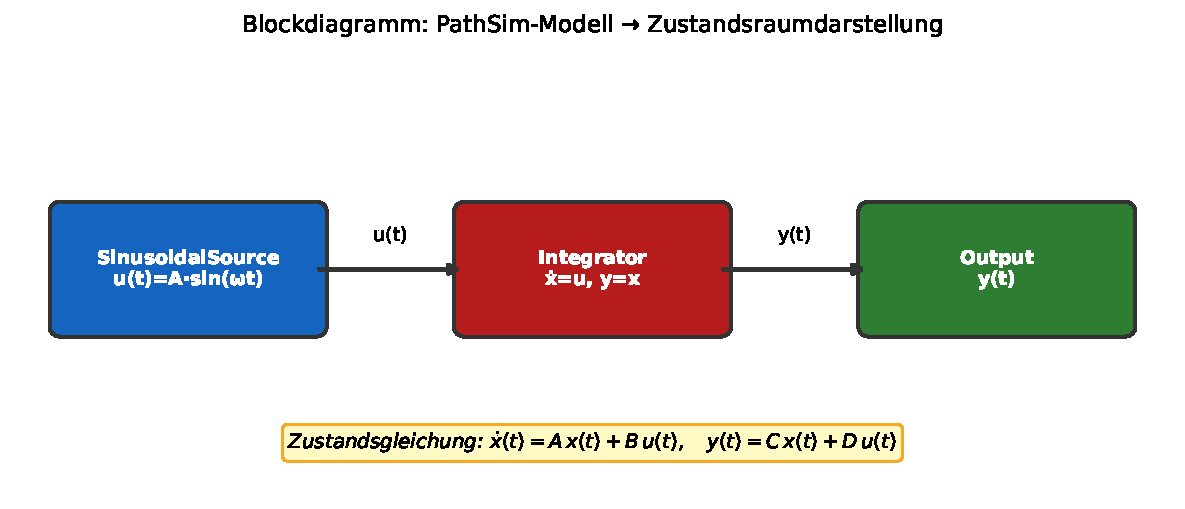
\includegraphics[width=0.88\textwidth]{plot_block.pdf}
  \caption{Blockdiagramm des PathSim-Modells und Zustandsraumdarstellung.}
  \label{fig:block}
\end{figure}


\section{Schlussfolgerungen und Ausblick}
\label{sec:schluss}


\subsection{Zusammenfassung der Hauptergebnisse}

Die vorliegende Arbeit hat folgende Kernaussagen bewiesen:

\begin{enumerate}[label=\textbf{S\arabic*.}]
  \item \textbf{Strukturisomorphismus} (\Cref{thm:iso}): Jedes lineare PathSim-Modell
        ist äquivalent zu einem LTI-Zustandsraumsystem $(A,B,C,D)$.
  \item \textbf{Minimale Blockbasis -- Vollständigkeit} (\Cref{thm:vollstaendig}):
        Die Menge $\mathcal{B}^* = \{\texttt{Integrator}, \texttt{Gain},
        \texttt{Adder}\}$ ist funktional vollständig für alle LTI-Systeme;
        jedes $(A,B,C,D)$ besitzt eine explizite Realisierung über $\mathcal{B}^*$
        via steuerbarer Normalform.
  \item \textbf{Minimale Blockbasis -- Minimalität} (\Cref{thm:minimal}):
        Keine echte Teilmenge von $\mathcal{B}^*$ ist vollständig. Jedes
        der drei Elemente ist primitiv und unersetzlich, in exakter Analogie
        zur Unzerlegbarkeit des $(A,B,C,D)$-Quadrupels.
  \item \textbf{Diskretisierungsordnungen} (\Cref{thm:euler,thm:rk4}): Euler liefert
        $\mathcal{O}(h)$, RK4 liefert $\mathcal{O}(h^4)$ globale Fehlerordnung.
  \item \textbf{Typsicherheit} (\Cref{thm:typesafe}): Der C99-Generator verletzt
        keine MISRA-C:2012 Typenregeln, wenn alle Signale als
        \texttt{model\_real\_t} typisiert werden.
  \item \textbf{Semantische Korrektheit} (\Cref{thm:correct}): Der generierte
        Code ist bit-genau äquivalent zur Python-Simulation.
  \item \textbf{Vollständigkeit} (\Cref{thm:complete}): Der Generator terminiert
        und erzeugt korrekten Code für jedes endliche Modell.
  \item \textbf{WCET-Schranke} (\Cref{thm:wcet}): $T_{\mathrm{WCET}} = \mathcal{O}(|V_B|)$,
        statisch analysierbar.
  \item \textbf{Determinismus} (\Cref{prop:det}): Der Code ist vollständig
        deterministisch und damit ISO~26262-kompatibel.
  \item \textbf{Subgraph Algorithmus -- Globale Korrektheit}
        (\Cref{thm:subgraph-global}):
        Der Subgraph Algorithmus erzeugt für jedes $K \in \{1,\ldots,|V_B|\}$
        eine gültige $K$-Zerlegung von $\mathcal{G}$, welche die
        Simulationssemantik bit-genau erhält, MISRA-konformen C99-Code
        für jede Partition liefert, die Fehlerordnungen der Diskretisierung
        konserviert und die parallele WCET auf
        $\mathcal{O}(|V_B|/K + \delta(\mathcal{P}) \cdot T_{\mathrm{sync}})$
        reduziert. Die optimale Partitionszahl beträgt
        $K^* = \lfloor\sqrt{|V_B|/(cD)}\rfloor$.
\end{enumerate}

\subsection{Neue Schlussfolgerungen}

\begin{itemize}
  \item \textbf{Schlussfolgerung A -- Formale Verifikationseignung:}
        Da der generierte Code deterministisch und schleifenfrei ist, eignet er
        sich direkt für formale Verifikationswerkzeuge (CBMC, Frama-C). Die
        formale Korrektheit der Simulation wird damit auf die Hardware
        übertragen.

  \item \textbf{Schlussfolgerung B -- Portabilität:}
        Durch den Einsatz von \texttt{stdint.h}-Typen und den Ausschluss
        implementierungsabhängiger Konstrukte ist der generierte Code auf
        allen Plattformen mit IEEE~754-konformem FPU portabel (ARM Cortex-M,
        RISC-V, x86).

  \item \textbf{Schlussfolgerung C -- Erweiterbarkeit auf nichtlineare Systeme:}
        Die Beweise in \Cref{sec:diskret,sec:synth} gelten analog für
        nichtlineare Blockklassen $\mathcal{F}_{\mathrm{nl}}$, sofern die
        Semantik-Abbildung $\llbracket \beta \rrbracket$ Lipschitz-stetig ist.

  \item \textbf{Schlussfolgerung D -- Optimale Schrittweite für Automotive:}
        Für typische AUTOSAR-Basistasks ($T_p = 1$~ms) empfiehlt \Cref{kor:stepsize}
        mit RK4 eine Schrittweite von $h \leq 10^{-3}/4 = 250~\mu$s bei
        Zielgenauigkeit $10^{-8}$.
\end{itemize}

\subsection{Ausblick}

Die vorliegende Arbeit schafft den formalen Unterbau für eine
zertifizierungsfähige Toolchain, die Blockdiagramm-Modelle in
MISRA-konformen eingebetteten C-Code überführt. Gleichzeitig öffnet sie
eine Vielzahl von Forschungsrichtungen, die die hier bewiesenen Ergebnisse
vertiefen, verallgemeinern und praktisch nutzbar machen. Die folgenden
Kapitel beleuchten die wichtigsten davon im Detail.

\subsubsection{Erweiterung der Blockbasis auf nichtlineare Systeme}

Der in \Cref{sec:basis} bewiesene Minimalitätssatz gilt für die Klasse der
LTI-Systeme. Eine zentrale offene Frage ist die Charakterisierung der
minimalen Blockbasis für \emph{nichtlineare} dynamische Systeme der Form
$\dot{x} = f(x, u)$, $y = g(x, u)$, wobei $f, g$ beliebig glatte
Abbildungen sind.

Sobald nichtlineare Blöcke wie \texttt{Multiplier} ($y = u_1 \cdot u_2$),
\texttt{Saturation}, \texttt{Abs} oder \texttt{LookupTable} eingeführt
werden, wird die Frage nach der minimalen Basis zu einem algebraischen
Strukturproblem. Für \emph{polynomiale Systeme} $\dot{x} = p(x, u)$
erwartet man: die Menge
$\mathcal{B}^*_{\mathrm{poly}} = \mathcal{B}^* \cup \{\texttt{Multiplier}\}$
ist vollständig, da Polynome durch Multiplikatoren und Addierer erzeugt
werden können (vgl.\ Weierstraß-Approximationssatz). Die Minimalität von
\texttt{Multiplier} gegenüber $\mathcal{B}^*$ ist zu beweisen: Es ist zu
zeigen, dass $y = u_1 \cdot u_2$ nicht bit-genau durch eine endliche
Schaltung aus Integratoren, Gains und Addierern simulierbar ist.

Für allgemein-glatte nichtlineare Systeme (z.\,B.\ $f(x) = \sin(x)$, wie
beim \texttt{Sinus}-Block selbst) würden transzendente Funktionsblöcke
benötigt. Hier stellt sich die Frage nach einer
\emph{universellen Approximationsbasis}: Analog zu universellen
Approximatoren (neuronale Netzwerke, Fourier-Reihen) könnte eine
parametrische minimale Familie von Blockklassen existieren, mit der jede
Lipschitz-stetige Dynamik bis auf $\varepsilon > 0$ approximiert werden kann.

\subsubsection{Erweiterung der Blockbasis auf zeitdiskrete Domäne}

In der zeitdiskreten Domäne (Differenzengleichungen
$x_{k+1} = A_d\,x_k + B_d\,u_k$) ist kein \texttt{Integrator} vorhanden.
Stattdessen hält ein \texttt{UnitDelay}-Block den Zustand um einen
Zeitschritt zurück: $y_k = x_{k-1}$. Ein unmittelbares Korollar aus
\Cref{thm:minimal} ist zu formulieren und zu beweisen:

\begin{quote}
\textit{Die minimale Blockbasis für zeitdiskrete LTI-Systeme ist gegeben durch $\mathcal{B}^*_d$ mit $\mathcal{B}^*_d = \{\texttt{UnitDelay},\;\texttt{Gain},\;\texttt{Adder}\}$,
wobei \texttt{UnitDelay} die Rolle des \texttt{Integrators} übernimmt.}
\end{quote}

Der Beweis verläuft vollständig analog zu \Cref{thm:minimal} und ist
strukturell identisch: Ohne \texttt{UnitDelay} sind nur statische
Abbildungen realisierbar; ohne \texttt{Gain} nur Systeme mit Einträgen in
$\{0,+1\}$; ohne \texttt{Adder} nur Systeme mit Fan-in~$\leq 1$.

Darüber hinaus liefert die formale Äquivalenz $\texttt{Integrator}
\leftrightarrow \texttt{UnitDelay}$ eine einheitliche Theorie für
gemischt kontinuierlich/diskrete (sampled-data) Systeme, bei denen
kontinuierliche und diskrete Signalpfade an Abtastinstanzen gekoppelt sind.

\subsubsection{Multirate-Systeme und Rate-Transition}

In Automotive-Anwendungen laufen Regelkreise typischerweise mit
verschiedenen Abtastraten: ABS und Lenkung bei $100\,\mu$s--$10$~ms,
Motorsteuerung bei $1$~ms, übergeordnete Fahrstrategien bei $100$~ms.
PathSim soll um \emph{Multirate-Fähigkeiten} erweitert werden:

\begin{itemize}
  \item \emph{Rate-Transition-Blöcke} puffern Signale an Subsystemgrenzen
        unterschiedlicher Abtastfrequenzen. Zu untersuchen ist der Einfluss
        der Hold-Interpolation (Zero-Order-Hold vs.\ First-Order-Hold) auf
        Stabilität und Approximationsgüte: Ein ZOH zwischen Subsystemen mit
        Raten $f_1 < f_2$ führt einen Haltestufenfehler der Ordnung
        $\mathcal{O}(1/f_1)$ ein.
  \item Die Minimalitätsfrage aus \Cref{sec:basis} ändert sich in der
        Multirate-Domäne: Ein \texttt{RateTransition}-Block ist
        \emph{nicht} durch $\mathcal{B}^*$ erzeugbar, ohne die
        Taktdomäne zu verlassen. Er bildet damit ein viertes, notwendiges
        Basiselement $\mathcal{B}^*_{\mathrm{mr}} = \mathcal{B}^* \cup
        \{\texttt{RateTransition}\}$ für Multirate-Systeme.
  \item Rein zeitdiskrete Subsysteme können ohne Diskretisierungsfehler
        kodiert werden und erfordern keinen Integrator -- ein direkter
        C99-Datenpfad \texttt{state[k+1] = A*state[k] + B*u[k]} wird generiert.
\end{itemize}

\subsubsection{Formale Verifikation des generierten Codes}

Die Beweise in \Cref{sec:synth} belegen semantische Korrektheit im
mathematischen Sinne. Ein unverzichtbarer Folgeschritt für
ASIL-C/D-Zertifizierungen ist die \emph{formale Verifikation} des
generierten C-Codes mit automatisierten Werkzeugen:

\begin{itemize}
  \item \textbf{CBMC (Bounded Model Checker):} CBMC kodiert für einen
        endlichen Ausführungshorizont $k$ die Eigenschaft
        $x_k^\mathcal{C} = x_k^{PS}$ als SMT-Formel und kann sie
        automatisch prüfen. Da der generierte Code schleifenfrei ist
        (\Cref{thm:wcet}), entfällt das Entfaltungsproblem; die Formel
        hat Größe $\mathcal{O}(|V_B| \cdot k)$. Eine integrierte
        Pipeline PathSim-Modell $\to$ C-Code $\to$ CBMC-Korrektheitsnachweis
        wäre unmittelbar realisierbar.

  \item \textbf{Frama-C mit WP-Plugin:} Der Weakest-Precondition-Calculus
        von Frama-C erlaubt deduktive Verifikation mit ACSL-Annotierungen.
        Ein automatischer Annotierungsgenerator könnte aus dem PathSim-Modell
        direkt Vor-/Nachbedingungen und Laufzeitschranken für jede generierte
        C-Funktion erzeugen. Für beschränkte Eingaben
        $\|u\|_\infty \leq U_{\max}$ sind Schranken $\|x(t)\|_\infty$
        über Systemmatrizen analytisch herleitbar (via Grönwall-Lemma) und
        als ACSL-Annotierungen codierbar, was Überlauf-Freiheit formal
        beweisbar macht.

  \item \textbf{Isabelle/HOL oder Lean~4:} Langfristig wäre eine
        vollständige Formalisierung des gesamten Beweisapparats dieser
        Arbeit -- insbesondere
        \Cref{thm:iso,thm:vollstaendig,thm:minimal,thm:correct} -- in
        einem interaktiven Theorembeweiser erstrebenswert. Ein
        maschinengeprüfter Korrektheitsbeweis bildet in
        ISO\,26262-ASIL-D-Audits ein entscheidendes Argument.
\end{itemize}

\subsubsection{Erweiterung auf nichtlineare und hybride Systeme}

Die Ergebnisse in \Cref{sec:diskret,sec:synth} setzen Linearität oder
zumindest globale Lipschitz-Stetigkeit voraus. Zwei wichtige
Erweiterungsrichtungen sind:

\begin{itemize}
  \item \emph{Nichtlineare stetige Systeme:} Die Konvergenzbeweise für
        Euler (\Cref{thm:euler}) und RK4 (\Cref{thm:rk4}) übertragen
        sich unmittelbar auf nichtlineare $f \in \mathcal{C}^5$, da sie
        nur globale Lipschitz-Stetigkeit voraussetzen. Zu erarbeiten ist
        ein allgemeiner Realisierungssatz, der \Cref{thm:iso} für
        nichtlineare Blockklassen ersetzt.

  \item \emph{Steife Systeme:} Systeme mit stark unterschiedlichen
        Zeitkonstanten (Steifheit $\kappa(A) := \lambda_{\max}/\lambda_{\min}
        \gg 1$) erfordern implizite Integrationsverfahren
        (Trapezregel, Radau-IIA). Der generierte Code muss dann
        iterative Gleichungslöser (Newton-Iteration) einschließen,
        was die WCET-Schranke von $\mathcal{O}(|V_B|)$ auf
        $\mathcal{O}(|V_B| \cdot \kappa_{\max})$ ändert, wobei
        $\kappa_{\max}$ die maximale Newton-Iterationsanzahl ist.

  \item \emph{Hybride Systeme:} PathSim-Modelle mit
        \texttt{Switch}-Blöcken führen bedingte Ausführungspfade ein
        (if-else im generierten Code), die MISRA-Regeln~15.x tangieren.
        Zenonische Chattering-Phänomene und Zustandsresets beim
        Modenwechsel müssen formal ausgeschlossen werden; eine
        Erweiterung des Isomorphismussatzes auf hybride Automaten
        ist anzustreben.
\end{itemize}

\subsubsection{Automatische Modellreduktion}

Große PathSim-Modelle (z.\,B.\ Gesamtfahrzeugmodelle mit $n > 10^3$
Zuständen) sind für Echtzeit-Embedded-Targets oft zu komplex. Automatische
Modellreduktion bietet hier systematische Abhilfe:

\begin{itemize}
  \item \emph{Balancierte Truncation (BRT):} Aus dem durch PathSim
        extrahierten LTI-System $(A, B, C, D)$ werden Steuer- und
        Beobachtbarkeits-Gramiane $W_c$, $W_o$ berechnet; Zustände mit
        kleinen Hankel-Singulärwerten $\sigma_{r+1} \leq \ldots \leq
        \sigma_n$ werden abgeschnitten. Der Approximationsfehler ist
        beschränkt durch
        \[
          \|y - y_{\mathrm{red}}\|_{\mathcal{H}_\infty}
          \leq 2\sum_{k=r+1}^n \sigma_k.
        \]
        Der PathSim-Codegenerator könnte das reduzierte System
        $(A_r, B_r, C_r, D_r) \in \mathbb{R}^{r \times r}$ direkt als
        C99-Code ausgeben.

  \item \emph{Proper Orthogonal Decomposition (POD):} Für nichtlineare
        Modelle bietet der Snapshot-basierte ROM-Ansatz eine Alternative;
        PathSim-Simulationen erzeugen die Trainings-Snapshots.

  \item \emph{Reduktions-Zertifikat:} Ein formal bewiesenes
        Fehlerszertifikat der Form $\|y - y_r\|_{\mathcal{L}^2} \leq
        \varepsilon_r$ für gegebene Eingabeklassen wäre als
        Erweiterung von \Cref{thm:correct} anzustreben.
\end{itemize}

\subsubsection{Quantisierung und Festkomma-Arithmetik}

Für kostengünstige Mikrocontroller ohne FPU (z.\,B.\ ARM Cortex-M0/M0+)
ist Festkomma-Arithmetik (Q-Format) erforderlich. Der Codegenerator
müsste um einen \emph{Quantisierungs-Pass} erweitert werden:

\begin{itemize}
  \item \emph{Skalierungsanalyse:} Für jeden Signalpfad muss der
        Wertebereich zur Kompilierzeit abgeschätzt werden, um optimale
        Q-Formatpositionen zu wählen und Über- bzw.\ Unterlauf zu
        verhindern.

  \item \emph{Fehler-Propagationstheorem:} Der Gesamtfehler
        $e_N^Q$ durch Quantisierung und Diskretisierung gemeinsam erfüllt
        \[
          e_N^Q \;\leq\; e_N^{\mathrm{diskret}}
          + \frac{N \cdot 2^{-Q}}{2L}\bigl(e^{LT}-1\bigr),
        \]
        wobei $L$ die Lipschitz-Konstante des Systems, $Q$ die
        Nachkommastellen-Wortlänge und $N = T/h$ die Schrittanzahl ist.

  \item \emph{Word-Length-Optimizer:} Ein automatischer Optimierer, der
        für gegebene Genauigkeitsanforderung $\varepsilon_Q$ die minimale
        Wortlänge berechnet und dabei Energieverbrauch (kürzere Typen
        $\to$ geringerer Aufwand) gegen Präzision abwägt, ist als
        integriertes Tool des PathSim-Generators denkbar.
\end{itemize}

\subsubsection{Vollständige ISO-26262-ASIL-D-Toolchain}

Die vorliegende Arbeit erfüllt die formalen Anforderungen für ASIL-B/C.
Eine vollständige ASIL-D-Zertifizierung erfordert zusätzlich:

\begin{itemize}
  \item \emph{Tool Qualification (TCL-3) nach Part~8:} Der PathSim-Codegenerator
        muss als Software Tool der Klasse TCL-3 qualifiziert werden. Dies
        umfasst: systematische Testabdeckung nach MC/DC-Kriterium für
        den Generator selbst, eine Fehler-Auswirkungsanalyse aller
        Generator-Komponenten sowie Regressionstests, die die in dieser
        Arbeit bewiesenen formalen Eigenschaften empirisch bestätigen.

  \item \emph{FMEA/FTA der generierten Funktionen:} Für jede
        Model-Funktion sind Fehler-Moden-Effekt-Analysen und
        Fehlerbäume zu erstellen, die zeigen, dass kein Single-Point-Fault
        zur Verletzung einer Sicherheitsanforderung führt.

  \item \emph{Back-to-Back-Test:} Die in \Cref{thm:correct} bewiesene
        bit-genaue Äquivalenz zwischen PathSim-Simulation und C-Code muss
        durch eine ausreichende Anzahl von Testfällen (Äquivalenzklassen
        des Eingaberaums) empirisch bestätigt werden -- der formale
        Beweis allein ist in ISO-26262-Audits nicht hinreichend.
\end{itemize}

\subsubsection{Parallele Codegenerierung für Mehrkernsysteme}

Für hochperformante Zielarchitekturen (z.\,B.\ Infineon AURIX TC4xx,
PYMCA-8) mit mehreren unabhängigen RISC-V-Kernen bietet die azyklische
Graphstruktur von PathSim-Modellen direkte Parallelisierungspotentiale:

\begin{itemize}
  \item \emph{Graphpartitionierung:} Der Subgraph Algorithmus
        \cite{subgraph2026} partitioniert $\mathcal{G}$ in $K$ Teilgraphen
        $\mathcal{G}_1, \ldots, \mathcal{G}_K$, sodass
        Kommunikationskosten minimiert und Rechenlast gleichmäßig
        verteilt werden. Die vollständige formale Theorie des Subgraph
        Algorithmus -- einschließlich Existenz- und Semantikerhaltungssatz,
        kompositionaler Korrektheit, MISRA-Typsicherheit und WCET-Analyse --
        ist in \Cref{sec:subgraph} ausgeführt und bewiesen.
        Insbesondere wurde in \Cref{thm:subgraph-global} gezeigt:
        Die parallele Ausführung der $K$ Partitionsfunktionen in
        topologischer Reihenfolge (\Cref{thm:sempreserve}) liefert
        bit-genau dasselbe Ergebnis wie die sequenzielle Auswertung
        (\Cref{thm:comp-correct}).

  \item \emph{Datenkonsistenz:} Signale, die Teilgraphgrenzen
        überqueren, erfordern Synchronisationsmechanismen (Mutex,
        Lock-Free-Puffer). MISRA-C~2023 bietet erste Richtlinien für
        Multithread-C, die in den Generator integriert werden müssten.

  \item \emph{Parallele WCET:} Die parallele WCET ist nicht trivial
        aus Einzel-WCET-Werten berechenbar -- Cache-Thrashing,
        Busbandbreiten und Synchronisations-Overhead müssen durch
        Modelle wie SymTA/S oder Compositional Performance Analysis
        erfasst werden.
\end{itemize}

\subsubsection{Subgraph Algorithmus: Weiterführende Forschungsrichtungen}
\label{subsubsec:subgraph-future}

Das in \Cref{sec:subgraph} vollständig formalisierte und bewiesene
Fundament des Subgraph Algorithmus eröffnet eine breite, tiefe
Forschungslandschaft, die weit über die in dieser Arbeit behandelten
Aspekte hinausgeht. Die folgenden Kapitel skizzieren die wichtigsten
offenen Fragen und Erweiterungsrichtungen mit konkreten Ansatzpunkten
für formale Beweise und Implementierungen.

\paragraph{Adaptiver Subgraph Algorithmus mit dynamischer Repartitionierung.}
Die in \Cref{alg:subgraph} beschriebene Zerlegung ist \emph{statisch}:
Sie wird einmal zur Kompilierzeit aus dem Blockgraphen berechnet und
fixiert. In der Praxis variieren jedoch die Rechenlasten einzelner
Partitionen zur Laufzeit -- etwa wenn nichtlineare Blöcke durch
iterative Newton-Schritte ausgewertet werden und die Anzahl der
Iterationen von der aktuellen Systemtrajektorie abhängt.

Eine zukünftige Erweiterung, der \emph{adaptive Subgraph Algorithmus},
verwaltet zur Laufzeit ein \emph{Lastprofil}
$\ell_i^{(k)} \in \mathbb{R}_{>0}$ pro Partition $i$ und Zeitschritt $k$.
Auf Basis einer gleitenden Mittelwert-Schätzung der tatsächlichen
Ausführungszeiten $\hat{C}_i^{(k)}$ wird entschieden, ob eine
Repartitionierung vorteilhaft ist:
\[
  \text{Repartitioniere, falls} \quad
  \max_i \hat{C}_i^{(k)} - \min_j \hat{C}_j^{(k)}
  > \theta \cdot T_{\mathrm{sync}},
\]
wobei $\theta > 0$ ein einstellbarer Schwellenwert ist. Die formalen
Beweise aus \Cref{thm:sempreserve,thm:comp-correct} müssen auf das
adaptive Szenario erweitert werden: Zu zeigen ist, dass eine
Repartitionierung während der Simulation -- ausgerichtet an einem
Synchronisationspunkt -- die semantische Erhaltung nicht verletzt.
Entscheidend ist dabei die korrekte Übergabe aller Zustandsvariablen
$x_i(t)$ an die neue Partition, d.\,h.\ eine bijektive Abbildung
der alten auf die neue Zustandsverteilung. Formell muss eine
\emph{Migrationsabbildung}
\[
  \phi : (V_{B,1}^{\text{alt}},\ldots,V_{B,K}^{\text{alt}})
  \longrightarrow
  (V_{B,1}^{\text{neu}},\ldots,V_{B,K}^{\text{neu}})
\]
als Bijektion auf $V_B$ definiert und bewiesen werden, dass
$\phi$ die Lower-Block-Triangular-Kopplung von \Cref{thm:comp-iso}
erhält.

\paragraph{Subgraph Algorithmus für heterogene Prozessorarchitekturen.}
Der in \Cref{alg:subgraph} formulierte Balancierungsfaktor $\alpha$
setzt implizit homogene Prozessorkerne voraus, bei denen jeder Block
die gleiche Ausführungszeit $T_b$ benötigt. Moderne heterogene
Systeme (z.\,B.\ AURIX TC4xx mit Kombination aus
TriCore-Kernen, MCS-Kernen und Hardware-Beschleunigern) haben
stark unterschiedliche Block-Kosten je nach Zielarchitektur.

Eine Erweiterung auf \emph{gewichtete Zerlegung} definiert
Block-Kostenfunktionen $c : V_B \times \mathcal{P}_{\mathrm{arch}} \to \mathbb{R}_{>0}$,
wobei $\mathcal{P}_{\mathrm{arch}}$ die Menge der verfügbaren
Prozessortypen bezeichnet. Das Optimierungsproblem lautet:
\[
  \min_{V_{B,1},\ldots,V_{B,K}} \max_{i=1}^K \sum_{v \in V_{B,i}} c(v, P_i)
\]
unter den Nebenbedingungen der Zerlegungsvalidität (\Cref{def:kdecomp}).
Dies ist ein NP-hartes Partitionierungsproblem (verwandt mit dem
Bin-Packing-Problem), für das polynomielle Approximationsalgorithmen
mit bekannten Approximationsgarantien existieren (z.\,B.\ Longest-Processing-Time-Heuristik
mit Güte $4/3$). Für den Subgraph Algorithmus ist ein solcher
Approximationsbeweis im Kontext der PathSim-Graphstruktur zu
führen: Die besondere Struktur azyklischer Signalfluss-Graphen
erlaubt möglicherweise bessere Schranken als im allgemeinen Fall.

\paragraph{Kommunikationsmodell auf spezifischen Busarchitekturen.}
Die in \Cref{def:commEdge} eingeführte Kommunikationskante
abstrahiert die Inter-Partition-Kommunikation auf eine einzige
Kante ohne Kostenmodell. Für den Einsatz auf realen
Embedded-Systemen ist ein differenzierteres Kommunikationsmodell
unerlässlich.

Für AURIX TC4xx-Systeme mit Local Memory Bus (LMB) und
Bus Interface Unit gilt das Verzögerungsmodell
\[
  T_{\mathrm{comm}}(s) = T_{\mathrm{setup}} + \lceil s / W_{\mathrm{bus}} \rceil \cdot T_{\mathrm{cycle}},
\]
wobei $s$ die Nachrichtengröße in Bytes, $W_{\mathrm{bus}}$ die
Busbreite und $T_{\mathrm{cycle}}$ die Buszykluszeit bezeichnet.
Ein erweiterter Subgraph Algorithmus würde das
Kommunikationsprofil $\kappa(\mathcal{P})$ durch eine
\emph{gewichtete Schnittbreite}
\[
  \hat{\kappa}_w(\mathcal{P})
  = \sum_{(u,v) \in E_{\mathcal{P}}^{\mathrm{comm}}} T_{\mathrm{comm}}(s_{uv})
\]
ersetzen und die Zerlegung so wählen, dass $\hat{\kappa}_w(\mathcal{P})$
minimiert wird.

Zu beweisen wäre: Für PathSim-Modelle mit
$\mathrm{sizeof}(\texttt{model\_real\_t}) = 8$ Bytes und
$W_{\mathrm{bus}} = 64$ Bits gilt
$T_{\mathrm{comm}}(s_{uv}) = T_{\mathrm{setup}} + T_{\mathrm{cycle}}$
unabhängig von der Anzahl der Kommunikationssignale (da jedes Signal
exakt ein Busübertragungswort belegt). Diese Vereinfachung macht
$\hat{\kappa}_w(\mathcal{P}) \propto \kappa(\mathcal{P})$ und
erlaubt die Rückführung auf die ungewichtete normierte Schnittbreite
aus \Cref{def:edgecut}.

\paragraph{Integration des Subgraph Algorithmus mit der Echtzeit-Scheduling-Theorie.}
Die in \Cref{thm:subgraph-wcet,thm:par-schedule} bewiesenen
Schedulability-Kriterien setzen voraus, dass jede Partition als
eigenständiger periodischer Task modelliert wird. In der Praxis
sind die $K$ Partitionstasks jedoch \emph{abhängige Tasks} (dependent
tasks) mit bekannten Vorrangbedingungen (precedence constraints),
die durch den Subgraph-Abhängigkeitsgraph $\mathcal{D}(\mathcal{P})$
(\Cref{def:subdep}) vollständig spezifiziert sind.

Die Erweiterung auf \emph{Scheduling mit Vorrangbedingungen}
basiert auf dem Algorithmus von Leung und Whitehead \cite{liu1973}
sowie dem Critical-Path-Verfahren aus der Projektplanung.
Der \emph{kritische Pfad} ist der längste gewichtete Pfad
$\pi^* = (i_0, i_1, \ldots, i_{\delta})$ in $\mathcal{D}(\mathcal{P})$:
\[
  \mathrm{CP}(\mathcal{P})
  = \max_{\pi \text{ Pfad in } \mathcal{D}(\mathcal{P})}
    \sum_{i \in \pi} C_i + \delta(\mathcal{P}) \cdot T_{\mathrm{sync}}.
\]
Das \emph{Kritische-Pfad-Scheduling-Theorem für den Subgraph Algorithmus}
-- zu formulieren und zu beweisen als Ergänzung zu
\Cref{thm:par-schedule} -- lautet:

\begin{quote}
\textit{Das aus dem Subgraph Algorithmus erzeugte TaskSystem ist genau
dann schedulable mit Periode $T_p$, wenn
$\mathrm{CP}(\mathcal{P}) \leq T_p$.}
\end{quote}

Der Beweis würde auf der Optimalität des EDF-Schedulers (Earliest
Deadline First) für abhängige Tasks beruhen und zeigen, dass der
kritische Pfad in $\mathcal{D}(\mathcal{P})$ die scharfe untere
Schranke der Ablaufplanungszeit darstellt. Diese Schranke ist
durch den Subgraph Algorithmus direkt minimierbar: Indem
$\delta(\mathcal{P})$ durch breitere statt tiefere Zerlegungen
reduziert wird, sinkt $\mathrm{CP}(\mathcal{P})$ auf Kosten
schlechterer Lastbalancierung. Das optimale $K^*$ aus
\Cref{kor:optimal-K} balanciert genau diesen Trade-off.

\paragraph{Subgraph Algorithmus für nichtlineare und hybride PathSim-Modelle.}
Die formalen Beweise in \Cref{sec:subgraph} setzen
$\mathcal{G} \in \mathcal{F}_{\mathrm{lin}}$ voraus, d.\,h.\ alle Blöcke
sind linear. Eine fundamentale Erweiterungsrichtung ist die Anwendung
des Subgraph Algorithmus auf nichtlineare Blockklassen
$\mathcal{F}_{\mathrm{nl}} \supset \mathcal{F}_{\mathrm{lin}}$.

\emph{Nichtlineare Signalfluss-Graphen:}
Für nichtlineare Blöcke $\beta \in \mathcal{F}_{\mathrm{nl}}$ gilt die
Semantik-Abbildung $\llbracket \beta \rrbracket$ nicht mehr als lineare
Abbildung. Dennoch bleiben die graphentheoretischen Eigenschaften des
Subgraph Algorithmus -- Azyklizität, Vollständigkeit, Disjunktheit,
Vorwärtsbedingung (\Cref{def:kdecomp}) -- vollständig erhalten, da
sie ausschließlich auf der Kantenstruktur von $\mathcal{G}$ beruhen
und keine Kenntnis der Block-Semantik voraussetzen.

Das zu beweisende Theorem lautet:
\begin{quote}
\textit{Sei $\mathcal{G}$ ein azyklischer Signalfluss-Graph über
$\mathcal{F}_{\mathrm{nl}}$, und sei jede Block-Semantik
$\llbracket\beta\rrbracket$ Lipschitz-stetig mit Konstante $L_\beta$.
Dann erzeugt der Subgraph Algorithmus eine gültige $K$-Zerlegung
$\mathcal{P}$, und für die Fehlerfortpflanzung gilt:
$e_N \leq \sum_{i=1}^K \bigl(\frac{M_i h}{2L_i}(e^{L_i T}-1)\bigr) + \mathcal{O}(\kappa(\mathcal{P}) \cdot h)$.}
\end{quote}

\emph{Hybride Systeme:} Bei PathSim-Modellen mit
\texttt{Switch}-Blöcken entstehen datenabhängige Kanten
$(u,v) \in E_{\mathrm{cond}}$, die nur aktiv sind, wenn eine Bedingung
$\psi(s) = \mathrm{true}$ gilt. Der Subgraph Algorithmus muss in
diesem Fall \emph{konservativ} vorgehen: Bedingte Kanten werden als
immer aktiv behandelt, sodass die Vorwärtsbedingung (\Cref{def:kdecomp}(d))
stets erfüllt ist. Dies führt zu einer Überschätzung des
Kommunikationsaufwands, erhält aber semantische Korrektheit:
Für jeden Betriebsmodus $\psi(s)$ ist die erzeugte Zerlegung gültig.

Eine optimierte Variante analysiert die Bedingungsstruktur
$\psi(s)$ symbolisch und partitioniert den Zustandsraum in
Gebiete, in denen verschiedene Kanten aktiv sind. In jedem
Gebiet gilt dann eine andere optimale Zerlegung; ein
\emph{mode-aware Subgraph Algorithmus} würde zur Laufzeit zwischen
Zerlegungen umschalten. Die formale Korrektheit eines solchen
Ansatzes erfordert einen Beweis, der \Cref{thm:sempreserve} auf
stückweise-glatte Vektorfelder (vgl.\ Fülop--Csikász-Nagy-Lemma
für hybride Systeme) überträgt.

\paragraph{Optimale Partitionszahl und Zerlegungstiefe: Verfeinerung der Komplexitätsanalyse.}
\Cref{kor:optimal-K} liefert eine erste Schätzung $K^* =
\lfloor\sqrt{|V_B|/(cD)}\rfloor$ für die optimale Partitionszahl.
Diese Formel setzt voraus, dass
(a)~die Zerlegungstiefe $\delta(\mathcal{P})$ unabhängig von $K$ ist und
durch $D$ nach oben beschränkt werden kann, und
(b)~der Synchronisationsoverhead linear in $\delta(\mathcal{P})$ skaliert.

Beide Annahmen sind vereinfachend. Eine verfeinerte Analyse muss berücksichtigen:

\begin{itemize}[nosep]
  \item \emph{Tiefenabhängigkeit von $K$:} Da tiefere Zerlegungen
        (größeres $K$) tendenziell mehr Stufen in $\mathcal{D}(\mathcal{P})$
        erzeugen, gilt im Allgemeinen
        $\delta(\mathcal{P}^{(K)}) = \mathcal{O}(\log K)$ für
        gut balancierte Graphen. Für Pfadgraphen $\mathcal{G}$ (lineare
        Ketten) gilt sogar $\delta(\mathcal{P}^{(K)}) = K - 1$.
        Die genaue Abhängigkeit $\delta(\mathcal{P}^{(K)})$ von der
        Graphstruktur von $\mathcal{G}$ und $K$ ist eine offene Frage mit
        Antworten, die direkt die optimale $K$-Wahl verfeinern.

  \item \emph{Nichtlinearer Synchronisationsoverhead:} In NUMA-Architekturen
        wächst $T_{\mathrm{sync}}$ mit dem Abstand zweier Kerne im
        Speicherhierarchiebaum. Ein NUMA-bewusstes Kommunikationsmodell
        würde $T_{\mathrm{sync}}(i,j) = f(d(P_i, P_j))$ einführen
        (wobei $d$ die Distanz im NUMA-Baum ist) und die optimale
        Zerlegung so anpassen, dass kommunizierende Partitionen auf
        topologisch benachbarte Kerne abgebildet werden -- ein
        kombiniertes Graph-Partitionierungs- und
        Prozessor-Zuweisungsproblem.

  \item \emph{Empirische Validierung des Modells:} Die
        Schranken aus \Cref{thm:subgraph-wcet,kor:optimal-K} sind
        analytisch; sie müssen durch systematische Messungen auf
        realer Hardware (ARM Cortex-A, RISC-V, TriCore) validiert
        werden. Insbesondere die Konstante $c$ (Verhältnis
        Synchronisationszeit zu Block-Ausführungszeit) ist
        plattformspezifisch und beeinflusst $K^*$ stark.
\end{itemize}

\paragraph{Subgraph Algorithmus und modellbasierte Diagnose.}
Eine überraschende Anwendung des Subgraph Algorithmus jenseits der
Codegenerierung liegt im Bereich der \emph{modellbasierten Online-Diagnose}
für eingebettete Systeme. In einem Diagnosesystem werden in jedem
Zeitschritt Modell-Ausgaben $y_{\mathcal{G}}(t)$ mit gemessenen
Ausgaben $y_{\mathrm{meas}}(t)$ verglichen; Abweichungen signalisieren
Fehler. Der Subgraph Algorithmus ermöglicht dabei eine
\emph{fehlerregion-sensitive Zerlegung}:

\begin{itemize}[nosep]
  \item Partitioniere $\mathcal{G}$ so, dass jede sicherheitskritische
        Zustandsvariable $x_j$ (z.\,B.\ Bremsdruck, Lenkwinkel) in
        einer dedizierten Partition mit hoher Priorität liegt.

  \item Das Diagnosesystem muss nur die Ausgaben $y_i(t)$ der
        sicherheitskritischen Partitionen hochfrequent überwachen
        ($f_{\mathrm{diag},i} \gg f_{\mathrm{diag},j}$ für unkritische
        Partitionen), was CPU-Last spart.

  \item Eine formale Theorie der \emph{Diagnosevollständigkeit}: Zu beweisen,
        dass jede Abweichung $\|y_{\mathrm{meas}}(t) - y_{\mathcal{G}}(t)\|
        > \varepsilon$ von mindestens einer Partition detektiert wird.
        Dies erfordert eine Erweiterung von \Cref{thm:sempreserve} auf
        Beobachtbarkeits-Argumente: Der Subgraph Algorithmus darf keine
        Partition erzeugen, die für die Ausgabe $y(t)$ unsichtbar ist.
\end{itemize}

\paragraph{Formale Verifikation des Subgraph Algorithmus selbst.}
Die Beweise in \Cref{sec:subgraph} sind mathematisch rigorose
Papierbeweise. Für sicherheitskritische Anwendungen (ASIL-D)
muss zusätzlich der Subgraph Algorithmus \emph{selbst}
formal verifiziert werden -- d.\,h.\ der Algorithmus-Code in
\Cref{alg:subgraph} sowie seine Python-Implementierung in PathSim.

\begin{itemize}[nosep]
  \item \emph{Lean-4-Formalisierung:} Die Sätze
        \Cref{thm:existence,thm:sempreserve,thm:comp-iso,%
        thm:comp-correct,thm:subgraph-global}
        sollen in Lean~4 maschinengeprüft bewiesen werden. Hierzu
        ist die gesamte Graphentheorie des Subgraph Algorithmus
        (Definitionen \ref{def:induced}--\ref{def:edgecut}) formal
        zu kodieren. Eine wesentliche Herausforderung ist die
        Formalisierung der Induktion über die Zerlegungstiefe
        $\delta(\mathcal{P})$ aus dem Beweis von \Cref{thm:sempreserve}.

  \item \emph{Isabelle/HOL -- Kahn-Topologiesort:} Der Kahn-Algorithmus
        \cite{kahn1962}, der im Subgraph Algorithmus zur topologischen
        Sortierung verwendet wird, ist in HOL4 und Isabelle/HOL
        formal verifiziert. Die Verbindung dieser bestehenden
        Verifikationen mit den Korrektheitseigenschaften des Subgraph
        Algorithmus könnte den Beweisaufwand erheblich reduzieren.

  \item \emph{CBMC-Verifikation der Python-Implementierung:} Die
        Python-Implementierung des Subgraph Algorithmus in PathSim
        könnte über CFFI nach C transpiliert und mit CBMC auf
        Zustandsinvarianten (\Cref{def:kdecomp}(a)--(d)) geprüft
        werden: insbesondere auf Vollständigkeit und Disjunktheit
        der erzeugten Partitionen sowie auf Azyklizität des
        Subgraph-Abhängigkeitsgraphen.
\end{itemize}

\paragraph{Subgraph Algorithmus und Modellreduktion.}
Eine synergetische Verbindung besteht zwischen dem Subgraph Algorithmus
und automatischer Modellreduktion
(vgl.\ Kapitel zur automatischen Modellreduktion weiter oben):

Die Balancierte-Truncation-Methode (BRT) berechnet für das
System $(A, B, C, D)$ das reduzierte System
$(A_r, B_r, C_r, D_r) \in \mathbb{R}^{r \times r}$.
Der \emph{blockweise} Einsatz des Subgraph Algorithmus ermöglicht
eine hierarchisch strukturierte Modellreduktion:

\begin{enumerate}[label=(\roman*), nosep]
  \item Wende den Subgraph Algorithmus an, um $\mathcal{G}$ in $K$
        Partitionen zu zerlegen.
  \item Berechne für jede Partition $\mathcal{G}_i$ das Teilsystem
        $\Sigma_i = (A_i, B_i, C_i, D_i)$ via \Cref{thm:comp-iso}.
  \item Reduziere jedes Teilsystem $\Sigma_i$ unabhängig auf
        Ordnung $r_i < n_i$ durch BRT; erhalte $\Sigma_i^{(r_i)}$.
  \item Verbinde die reduzierten Teilsysteme über die
        Lower-Block-Triangular-Kopplung zu einem reduzierten
        Gesamtsystem der Ordnung $r = \sum_i r_i$.
\end{enumerate}

Der Approximationsfehler des hierarchisch reduzierten Systems
erfüllt nach der Dreiecksungleichung:
\[
  \|y - y_{\mathrm{red}}\|_{\mathcal{H}_\infty}
  \;\leq\; \sum_{i=1}^K
  2 \sum_{k=r_i+1}^{n_i} \sigma_k^{(i)},
\]
wobei $\sigma_k^{(i)}$ die Hankel-Singulärwerte des $i$-ten
Teilsystems sind. Diese Schranke ist typischerweise kleiner als
die durch direkte globale BRT erreichbare Schranke, da die
Teilsysteme jeweils eigenständige Eigenstruktures besitzen.
Ein vollständiger Beweis dieser Ungleichung ist eine offene Aufgabe
und bildet eine wichtige Brücke zwischen den in \Cref{sec:subgraph}
und \Cref{sec:schluss} entwickelten Theorien.

\paragraph{Mehrobjektive Optimierung der Zerlegungsqualität.}
Bisher wird der Subgraph Algorithmus mit einem einzigen Ziel genutzt:
minimale Rechenunausgewogenheit $\Delta(\mathcal{P})$. Reale
Embedded-Systeme erfordern jedoch ein mehrobjektives Optimierungsproblem:
\[
  \min_{\mathcal{P}} \Bigl(
    \underbrace{\Delta(\mathcal{P})}_{\text{Lastbalance}},\;
    \underbrace{\kappa(\mathcal{P})}_{\text{Kommunikation}},\;
    \underbrace{\delta(\mathcal{P})}_{\text{Tiefe/Latenz}},\;
    \underbrace{k_{\mathrm{cross}}(\mathcal{P})}_{\text{Speicherkohärenz}}
  \Bigr),
\]
wobei $k_{\mathrm{cross}}(\mathcal{P})$ die Anzahl der Cache-line-crossing
Kommunikationssignale (d.\,h.\ Signale, die auf Caches verschiedener
Kerne zugreifen) bezeichnet.

Dieses vektorielles Optimierungsproblem besitzt im Allgemeinen kein
einziges globales Minimum, sondern eine \emph{Pareto-Front}.
Für den Subgraph Algorithmus ist zu untersuchen:

\begin{itemize}[nosep]
  \item Existenz und Charakterisierung der Pareto-optimalen Zerlegungen
        als Funktion der Graphstruktur $\mathcal{G}$.
  \item Effizienz-Kompromisse: Für azyklische Graphen mit
        Bandstruktur (viele lokale Abhängigkeiten) ist
        $\delta(\mathcal{P})$ und $\kappa(\mathcal{P})$ gleichzeitig
        niedrig haltbar; für irregulär vernetzte Graphen existiert
        ein fundamentaler Widerspruch zwischen niedriger
        Kommunikation und niedriger Tiefe.
  \item Approximierbarkeit: Ist die Berechnung der Pareto-Front
        polynomial in $|V_B|$ und $K$, oder ist das Problem für
        allgemeine Graphen NP-schwer?
\end{itemize}

Selbst eine heuristische Annäherung an die Pareto-Front mittels
gewichteter Scalarisierung
$\min_{\mathcal{P}} (\alpha_1 \Delta + \alpha_2 \kappa + \alpha_3 \delta + \alpha_4 k_{\mathrm{cross}})$
für benutzerdefinierte Gewichte $\alpha_i \geq 0$ würde den
praktischen Nutzen des Subgraph Algorithmus erheblich steigern.

\paragraph{Subgraph Algorithmus und inkrementelle Codegenerierung.}
Die in \Cref{thm:comp-complete} bewiesene Vollständigkeit der
zerlegten Synthese setzt voraus, dass das gesamte Modell $\mathcal{G}$
neu übersetzt wird. In industrieller Modellentwicklung sind jedoch
iterative Modifikationen der Regel: typischerweise werden pro
Entwicklungsiteration nur wenige Blöcke $\Delta V_B \subseteq V_B$
hinzugefügt, entfernt oder parametrisch verändert.

Der \emph{inkrementelle Subgraph Algorithmus} nutzt die Zerlegungsstruktur
für effiziente Neusynthese:

\begin{enumerate}[label=(\roman*), nosep]
  \item \emph{Change-Impact-Analyse:} Bestimme alle Partitionen
        $\mathcal{P}_{\mathrm{dirty}} \subseteq \{1,\ldots,K\}$, deren
        Zustandsmenge $V_{B,i}$ direkt betroffen ist:
        $\mathcal{P}_{\mathrm{dirty}} = \{i : V_{B,i} \cap \Delta V_B \neq \emptyset\}$.

  \item \emph{Transitive Hülle:} Bestimme alle transitiv abhängigen
        Partitionen über den Abhängigkeitsgraphen:
        $\mathcal{P}_{\mathrm{dirty}}^* = \{j : \exists \text{ Pfad } i \to j
        \text{ in } \mathcal{D}(\mathcal{P}),\; i \in \mathcal{P}_{\mathrm{dirty}}\}$.

  \item \emph{Selektive Neusynthese:} Generiere neuen C-Code nur für
        $\mathcal{G}_j$ mit $j \in \mathcal{P}_{\mathrm{dirty}}^*$;
        der Code der unberührten Partitionen $\{1,\ldots,K\} \setminus
        \mathcal{P}_{\mathrm{dirty}}^*$ bleibt unverändert.
\end{enumerate}

Zu beweisen ist, dass die inkrementelle Neusynthese
\emph{semantisch äquivalent} zur vollständigen Neusynthese ist.
Formal muss gezeigt werden, dass das Ergebnis der inkrementellen
Codegenerierung identisch mit dem Ergebnis einer vollständigen
Anwendung von \Cref{alg:subgraph} und \Cref{thm:comp-complete}
auf das modifizierte Modell $\mathcal{G}' = (V \cup \Delta V, E \cup
\Delta E, \ldots)$ ist. Die Komplexität des inkrementellen Subgraph
Algorithmus beträgt $\mathcal{O}(|\mathcal{P}_{\mathrm{dirty}}^*| \cdot |V_B|/K)$,
was bei kleinen Änderungen ($|\Delta V_B| \ll |V_B|$) einen erheblichen
Speedup gegenüber vollständiger Neusynthese darstellt.

\paragraph{Theorie der optimalen Zerlegungstiefe und Bandbreite.}
Das Verhältnis zwischen Zerlegungstiefe $\delta(\mathcal{P})$ und
normierter Schnittbreite $\hat{\kappa}(\mathcal{P})$ unterliegt einem
strukturellen Widerspruch, der als \emph{Tiefe-Bandbreite-Dilemma}
bezeichnet werden kann:

\begin{itemize}[nosep]
  \item Eine geringe Tiefe $\delta(\mathcal{P})$ erfordert breite Partitionen,
        was zu hohem Kommunikationsaufwand $\kappa(\mathcal{P})$
        und damit hoher normierter Schnittbreite $\hat{\kappa}(\mathcal{P})$ führt.
  \item Eine geringe Schnittbreite $\hat{\kappa}(\mathcal{P})$ erfordert
        Partitionen entlang natürlicher Trennflächen des Graphen,
        was oft eine längere Abhängigkeitskette erzeugt.
\end{itemize}

Formal lautet die offene Frage: Für einen azyklischen Signalfluss-Graphen
$\mathcal{G}$ und eine $K$-Zerlegung -- wie lautet die untere Schranke
für das Produkt
\[
  \Phi(\mathcal{P}) = \delta(\mathcal{P}) \cdot \hat{\kappa}(\mathcal{P})?
\]
Existiert eine universelle Konstante $c_{\mathcal{G}} > 0$, sodass
$\Phi(\mathcal{P}) \geq c_{\mathcal{G}}$ für alle gültigen $K$-Zerlegungen
gilt? Das wäre ein Analogon zum Isoperimetrischen Ungleichung auf
Graphen (Cheeger-Ungleichung) und würde fundamentale Grenzen der
erreichbaren Parallelisierungseffizienz bei PathSim-Modellen etablieren.

\paragraph{Erweiterung des Subgraph Algorithmus auf algebraische Schleifen.}
Die Voraussetzung der Azyklizität (\Cref{def:kdecomp}(c)) schließt
Modelle mit algebraischen Schleifen aus. Algebraische Schleifen
entstehen in PathSim, wenn ein Signalpfad ohne Gedächtniselement
(ohne \texttt{Integrator}) einen Zykel im Graphen bildet; dies
geschieht z.\,B.\ bei impliziten algebraischen Gleichungssystemen
(differential-algebraische Gleichungen, DAE).

Für DAE-Systeme der Form $F(\dot{x}, x, u) = 0$ existieren
Lösungsverfahren (BDF-Methoden, Radau-IIA \cite{gear1971}), die
iterative Gleichungslöser verwenden. Der Subgraph Algorithmus
müsste in diesem Fall:

\begin{enumerate}[label=(\roman*), nosep]
  \item Zyklen im Graphen $\mathcal{G}$ identifizieren und als
        \emph{strongly connected components} (SCCs) zusammenfassen.
  \item Jede SCC als einen einzigen Block behandeln, der intern
        durch einen iterativen Gleichungslöser ausgewertet wird.
  \item Die resultierende SCC-Kondensation als azyklischen Graphen
        behandeln und darauf den Subgraph Algorithmus anwenden.
\end{enumerate}

Zu beweisen ist, dass diese Erweiterung die semantische Erhaltung
(\Cref{thm:sempreserve}) auf DAE-Systeme überträgt; der Beweis
erfordert, dass der iterative Gleichungslöser innerhalb jeder SCC
korrekt konvergiert und die Toleranzen konsistent mit den
Diskretisierungsfehlern aus \Cref{thm:subgraph-error} sind.

\paragraph{Subgraph Algorithmus für zeitkontinuierliche Compiler-Integration.}
Eine langfristige Vision ist die vollständige Integration des
Subgraph Algorithmus in einen modernen C-Compiler als
\emph{linkerübergreifende Interprozedural-Analyse}. Hierbei
würde der Compiler das Blockgraph-Modell nicht aus Python,
sondern direkt aus annotierten C-Quellen extrahieren:

\begin{lstlisting}[style=cstyle, caption={Annotiertes C-Format für den Subgraph Algorithmus}]
/* PathSim-Annotation: Blockgraph-Kanten fuer Subgraph Algorithmus */
__attribute__((pathsim_block(integrator, state="x1")))
static model_real_t integrate_x1(model_real_t xdot) {
    return x1 + DT * xdot;
}

__attribute__((pathsim_block(gain, param=OMEGA_N)))
static model_real_t gain_omegan(model_real_t in) {
    return OMEGA_N * in;
}
\end{lstlisting}

Der Compiler extrahiert aus diesen Annotierungen den Blockgraphen
$\mathcal{G}$, wendet den Subgraph Algorithmus an und distribuiert
die resultierenden Partitionen auf verfügbare Kerne -- ohne dass der
Entwickler explizit parallelisieren muss. Die Korrektheit dieses
Ansatzes entspräche einem automatischen Korrektheitsbeweis auf
Compilerebene: Der Compiler würde als \emph{zertifiziertes
Übersetzungswerkzeug} gelten, dessen Korrektheit direkt auf
\Cref{thm:subgraph-global} fußt.

Diese Vision verbindet Compilerbau, Graphentheorie und formale
Verifikation und bildet einen natürlichen Abschluss der in
\Cref{sec:subgraph} und \Cref{sec:synth} entwickelten Theorie.

\subsubsection{Erweitertes Typsystem: Vektorsignale und komplexe Zahlen}

Das in \Cref{sec:misra} entwickelte Typsystem beschränkt sich auf skalare
\texttt{model\_real\_t}-Signale. Praktische Anwendungen erfordern:

\begin{itemize}
  \item \emph{Vektorsignale:} Busse und Vektorknoten ($u \in \mathbb{R}^k$)
        müssen als typisierte Arrays dargestellt werden. Das MISRA-Typsystem
        muss um Array-Typen erweitert werden; Rule~18.x (Pointer/Array)
        tritt in den Vordergrund. Für Vektorsignale ist \Cref{thm:typesafe}
        neu zu formulieren und zu beweisen.

  \item \emph{Komplexwertige Signale:} Für Signalverarbeitungsanwendungen
        (FFT-Blöcke, I/Q-Demodulation) sind $z \in \mathbb{C}$ erforderlich.
        Da MISRA-C:2012 \texttt{\_Complex}-Typen nicht direkt unterstützt,
        müssten komplexe Zahlen als Struct $\{$\texttt{re}, \texttt{im}$\}$
        mit expliziten Rechenregeln implementiert werden -- ein vollständig
        neues Type-Safety-Theorem wäre notwendig.

  \item \emph{Matrixsignale für Mehrkörpersimulation:} Rotationsmatrizen
        $R \in \mathrm{SO}(3)$ und homogene Transformationsmatrizen
        $T \in \mathrm{SE}(3)$ als Signaltypen erfordern ein Typsystem,
        das Gruppenstruktur (Orthogonalität, $\det = 1$) als statisch
        verifizierbare Invariante kodiert.
\end{itemize}

\subsubsection{Lernbasierte Blockbibliotheken und KI-Integration}

Eine zukunftsweisende Erweiterung betrifft datengetriebene Modellkomponenten:

\begin{itemize}
  \item \emph{Physics-Informed Neural Networks (PINNs):} PINNs, die
        eine Differentialgleichung $\dot{x} = f(x,u)$ als Residuum im
        Loss kodieren, könnten als spezialisierte Integrator-Blöcke
        mit gelerntem Vektorfeld fungieren. Trainings- und
        Approximationsfehler müssen in die Fehleranalyse einbezogen
        werden.

  \item \emph{Symbolische Regression zur Blockbibliotheks-Erweiterung:}
        Mittels PySR könnten aus Messdaten automatisch neue Blockklassen
        $\beta \in \mathcal{F}$ mit formaler Semantik identifiziert
        werden, die sich anschließend -- ohne die Minimalität von
        $\mathcal{B}^*$ zu verletzen -- als abgeleitete (nicht-primitive)
        Klassen in PathSim integrieren lassen.
\end{itemize}

\subsubsection{Kompositionelle Korrektheit und Subsystem-Abstraktion}

Industrielle PathSim-Modelle sind hierarchisch strukturiert.
Zukünftige Arbeit sollte eine formale Theorie der
\emph{kompositionellen Korrektheit} entwickeln:

\begin{itemize}
  \item \emph{Subsystem-Blöcke:} Ein \texttt{Subsystem}-Block kapselt
        ein vollständiges PathSim-Modell $\mathcal{G}'$ als primitiven
        Block in $\mathcal{G}$. Korrektheit der Codegenerierung für
        $\mathcal{G}$ soll \emph{kompositional} aus der Korrektheit der
        Teilgraphen folgen -- formal basierend auf
        Assume-Guarantee-Reasoning.

  \item \emph{Parametrische Korrektheit:} Eine parameterräumliche
        Korrektheit -- ``Für alle $\mu \in \mathcal{P}$ gilt
        $y_{\mathcal{G}(\mu)}(t) = y_{\Sigma(\mu)}(t)$'' -- würde
        \Cref{thm:correct} zu einer Familie von Modellen verallgemeinern
        und wäre für model-in-the-loop Variationsanalysen bedeutsam.

  \item \emph{Inkrementelle Codegenerierung:} Bei kleinen
        Modifikationen an $\mathcal{G}$ (Parameteränderungen,
        Hinzufügen/Entfernen eines Blocks) sollte der Codegenerator
        nur den betroffenen Ausschnitt neu generieren. Ein
        Change-Impact-Analysealgorithmus auf dem Blockgraphen -- mit
        formaler Korrektheitsdefinition -- ist Gegenstand zukünftiger
        Untersuchungen.
\end{itemize}


\begin{thebibliography}{9}
\bibitem{pathsim2024}
  PathSim Development Team,
  \emph{PathSim: A Python-based Block Diagram Simulation Framework},
  \url{https://code.pathsim.org}, 2024.

\bibitem{misra2012}
  MISRA Consortium,
  \emph{MISRA-C:2012 -- Guidelines for the Use of the C Language in Critical Systems},
  3rd~ed., MIRA Ltd., 2012.

\bibitem{hairer1993}
  E.~Hairer, S.~P.~N{\o}rsett, G.~Wanner,
  \emph{Solving Ordinary Differential Equations I: Nonstiff Problems},
  2nd~ed., Springer, 1993.

\bibitem{iso26262}
  ISO,
  \emph{ISO~26262: Road Vehicles -- Functional Safety},
  2nd~ed., ISO, 2018.

\bibitem{kahn1962}
  A.~B.~Kahn,
  ``Topological sorting of large networks,''
  \emph{Communications of the ACM}, vol.~5, no.~11, pp.~558--562, 1962.

\bibitem{liu1973}
  C.~L.~Liu, J.~W.~Layland,
  ``Scheduling algorithms for multiprogramming in a hard-real-time environment,''
  \emph{Journal of the ACM}, vol.~20, no.~1, pp.~46--61, 1973.

\bibitem{subgraph2026}
Epp, S.,
\textit{Subgraph Algorithmus},
2026, Verfügbar bei \url{https://github.com/hjstephan86/science}.

\bibitem{chen1999}
  C.~T.~Chen,
  \emph{Linear System Theory and Design},
  3rd~ed., Oxford University Press, New York, 1999.

\bibitem{antsaklis2006}
  P.~J.~Antsaklis, A.~N.~Michel,
  \emph{A Linear Systems Primer},
  Birkhäuser, Boston, 2007.

\bibitem{brogan1991}
  W.~L.~Brogan,
  \emph{Modern Control System Theory and Design},
  2nd~ed., Prentice Hall, Englewood Cliffs, NJ, 1991.

\bibitem{sontag1998}
  E.~D.~Sontag,
  \emph{Mathematical Control Theory: Deterministic Finite-Dimensional Systems},
  2nd~ed., Springer, New York, 1998.

\bibitem{khalil2002}
  H.~K.~Khalil,
  \emph{Nonlinear Systems},
  3rd~ed., Prentice Hall, Upper Saddle River, NJ, 2002.

\bibitem{ascher1998}
  U.~M.~Ascher, L.~R.~Petzold,
  \emph{Computer Methods for Ordinary Differential Equations and Differential-Algebraic Equations},
  SIAM, Philadelphia, 1998.

\bibitem{butcher2008}
  J.~C.~Butcher,
  \emph{Numerical Methods for Ordinary Differential Equations},
  2nd~ed., Wiley, Chichester, 2008.

\bibitem{dormand1980}
  J.~R.~Dormand, P.~J.~Prince,
  ``A family of embedded Runge-Kutta formulae,''
  \emph{Journal of Computational and Applied Mathematics}, vol.~6, no.~1,
  pp.~19--26, 1980.

\bibitem{gear1971}
  C.~W.~Gear,
  \emph{Numerical Initial Value Problems in Ordinary Differential Equations},
  Prentice Hall, Englewood Cliffs, NJ, 1971.

\bibitem{mason1953}
  S.~J.~Mason,
  ``Feedback theory -- some properties of signal flow graphs,''
  \emph{Proceedings of the IRE}, vol.~41, no.~9, pp.~1144--1156, 1953.

\bibitem{coates1959}
  C.~L.~Coates,
  ``Flow-graph solutions of linear algebraic equations,''
  \emph{IRE Transactions on Circuit Theory}, vol.~6, no.~2, pp.~170--187, 1959.

\bibitem{kopetz2011}
  H.~Kopetz,
  \emph{Real-Time Systems: Design Principles for Distributed Embedded Applications},
  2nd~ed., Springer, New York, 2011.

\bibitem{lee2017}
  E.~A.~Lee, S.~A.~Seshia,
  \emph{Introduction to Embedded Systems: A Cyber-Physical Systems Approach},
  2nd~ed., MIT Press, Cambridge, MA, 2017.

\bibitem{iec61508}
  IEC,
  \emph{IEC~61508: Functional Safety of Electrical/Electronic/Programmable
  Electronic Safety-Related Systems},
  2nd~ed., IEC, Geneva, 2010.

\bibitem{hatton1995}
  L.~Hatton,
  \emph{Safer C: Developing Software for High-Integrity and Safety-Critical Systems},
  McGraw-Hill, New York, 1995.

\bibitem{storey1996}
  N.~Storey,
  \emph{Safety-Critical Computer Systems},
  Addison-Wesley, Harlow, 1996.

\bibitem{clarke1999}
  E.~M.~Clarke, O.~Grumberg, D.~Peled,
  \emph{Model Checking},
  MIT Press, Cambridge, MA, 1999.

\bibitem{cormen2009}
  T.~H.~Cormen, C.~E.~Leiserson, R.~L.~Rivest, C.~Stein,
  \emph{Introduction to Algorithms},
  3rd~ed., MIT Press, Cambridge, MA, 2009.

\bibitem{aho2006}
  A.~V.~Aho, M.~S.~Lam, R.~Sethi, J.~D.~Ullman,
  \emph{Compilers: Principles, Techniques, and Tools},
  2nd~ed., Addison-Wesley, Boston, 2006.

\bibitem{c99standard}
  ISO/IEC,
  \emph{ISO/IEC 9899:1999 -- Programming Languages -- C},
  ISO, Geneva, 1999.

\bibitem{ieee754-2019}
  IEEE,
  \emph{IEEE~754-2019: IEEE Standard for Floating-Point Arithmetic},
  IEEE, New York, 2019.

\bibitem{autosar2021}
  AUTOSAR Consortium,
  \emph{AUTOSAR Classic Platform -- Release R21-11},
  \url{https://www.autosar.org}, 2021.

\bibitem{barr2006}
  M.~Barr, A.~Massa,
  \emph{Programming Embedded Systems: With C and GNU Development Tools},
  2nd~ed., O'Reilly Media, Sebastopol, CA, 2006.

\bibitem{henzinger1996}
  T.~A.~Henzinger,
  ``The theory of hybrid automata,''
  \emph{Proceedings of the 11th Annual IEEE Symposium on Logic in Computer Science (LICS)},
  pp.~278--292, 1996.

\bibitem{griewank2008}
  A.~Griewank, A.~Walther,
  \emph{Evaluating Derivatives: Principles and Techniques of Algorithmic Differentiation},
  2nd~ed., SIAM, Philadelphia, 2008.

\bibitem{bernstein2009}
  D.~S.~Bernstein,
  \emph{Matrix Mathematics: Theory, Facts, and Formulas},
  2nd~ed., Princeton University Press, Princeton, NJ, 2009.

\end{thebibliography}

\end{document}
